\appendix
\chapter{Results for 3DLite}
\section{Mesh Visualization}
In Figure~\ref{fig:vis}, we visualize the 3D models processed with 3DLite. 
The first column is the original mesh reconstructed with VoxelHashing~\cite{niessner2013real} using camera poses from BundleFusion~\cite{dai2016bundlefusion}. 
The second column is a visualization of our plane fitting algorithm. 
The third column shows our results of plane extrapolation. 
For the last column, we show the final results produced from our algorithm.
\begin{figure*}
    \centering
    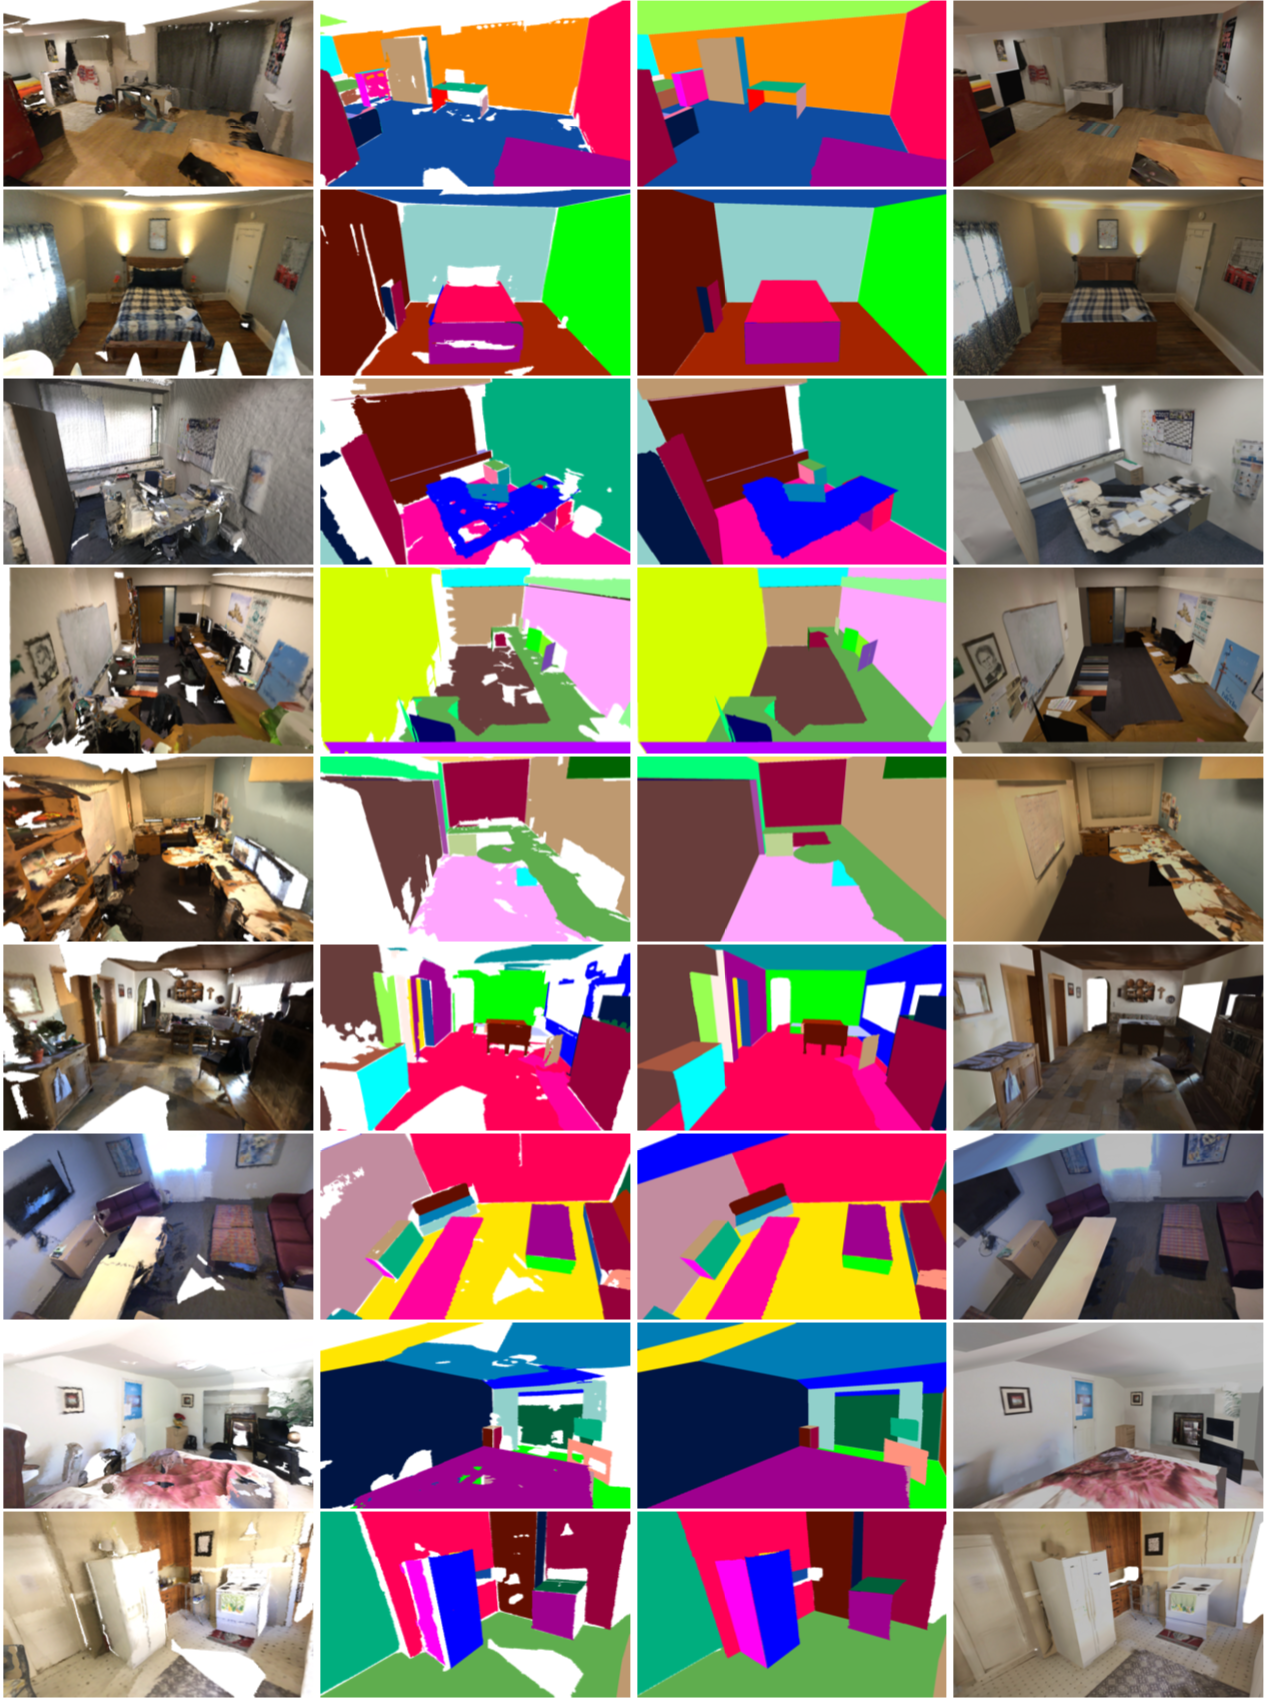
\includegraphics[width=0.9\linewidth]{3dlite/fig22.png}
    \caption{Mesh Visualization.  The first column is the original mesh reconstructed with VoxelHashing~\cite{niessner2013real} using camera poses from BundleFusion~\cite{dai2016bundlefusion}. The second column is a visualization of our plane fitting algorithm. The third column shows our results of plane extrapolation. For the last column, we show the final results produced from our algorithm.}
    \label{fig:vis}
\end{figure*}

\chapter{More TextureNet Experiments}
\section{Comparison to 2D Convolution on Texture Atlas}

We did an additional experiment to compare our convolution operator with traditional image convolutions on a color texture atlas created with a standard UV parameterization, as shown in Figure~\ref{fig:texturenet-textureimage}. For this experiment, we trained a state-of-the-art network (DenseNet~\cite{huang2017densely}) on the semantic labels mapped to the texture map image.  The results with that method are not very good -- the mean class IoU is only 12.2\%, as compared to 56.6\% with our method.  We conjecture the reason is that UV parameterizations are not consistent across examples and convolutions are affected by texture seams. 

\begin{figure}[h]
    \centering
    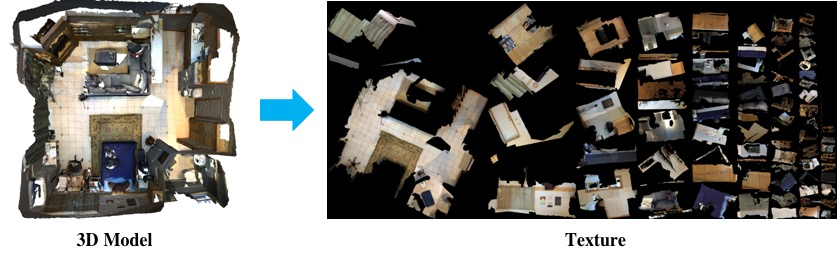
\includegraphics[width=\linewidth]{texturenet/diagram/texture.jpg}
    \caption{An example of the texture image.}
    \label{fig:texturenet-textureimage}
\end{figure}

\jw{We additionally tried an as-rigid-as-possible parameterization, which achieves 16.8 IoU (ours is 58.1).
The poor performance is mainly due to convolutions over regions with seams, large distortions, and inconsistent orientations -- i.e., the main problems that our 4-rosy approach aims to resolve.}

%%%%%%%%%%%%%%%%%%%%%%%%%%%%%%%%%%%%%%%%%%%%%%%%%%%%%%%%
\section{Evaluation of Neighborhood Selection Methods}

The next experiment tests whether the geodesic neighborhoods used by TextureNet convolutional operators are better than volumetric ones used by PointNet++.   To test this, we compare the performance of the original PointNet++ network which takes the Euclidean ball as the neighborhood, with slightly modified versions which take a cuboid or our geodesic patch as a neighborhood. As shown in Table~\ref{tab:texturenet-neighbor}, the geodesic patch achieves a slightly higher score. This might be due to the reason that it is easier for the network to learn the boundary on the 2D subsurface than on the 3D space.

\begin{table*}[h]
    \centering
    \scriptsize
    \tabcolsep=0.04cm
    \begin{tabular}{|c|c|c|c|c|c|c|c|c|c|c|c|c|c|c|c|c|c|c|c|c|c|c|}
        \hline
        Input & wall & floor & cab & bed & chair & sofa & table & door & wind & bkshf & pic & cntr & desk & curt & fridg & show & toil & sink & bath & other & ave\\
        \hline
        Ball & \textbf{68.1} & \textbf{96.2} & 34.9 & 41.2 & 61.8 & 43.0 & 24.1 & 5.0 & 19.2 & 41.7 & 0.0 & 4.7 & 11.8 & 17.7 & 20.1 & 30.8 & 72.2 & 43.7 & 55.2 & 8.7 & 35.0 \\
        \hline
        Cube1 & 65.3 & 95.8 & 29.0 & 57.0 & 61.2 & 46.2 & 42.7 & 17.8 & 11.8 & 35.1 & 0.7 & \textbf{37.3} & \textbf{39.0} & 55.4 & 8.5 & 43.9 & 63.0 & 30.6 & 52.4 & 15.0 & 40.4 \\
        \hline
        Cube2 & 58.7 & 90.0 & \textbf{61.6} & \textbf{62.6} & 59.3 & 50.4 & 40.2 & 31.3 & 15.1 & 45.6 & 1.9 & 29.4 & 23.9 & 53.1 & 18.2 & 41.8 & 81.7 & 34.1 & 51.8 & 25.2 & 43.9 \\
        \hline
        Cube4 & 32.7 & 86.8 & 59.6 & 49.1 & 51.3 & 33.7 & 30.0 & 27.0 & 11.8 & 33.8 & 0.9 & 20.9 & 19.5 & 40.3 & 15.1 & 29.8 & 54.1 & 27.7 & 41.7 & 17.0 & 34.2 \\
        \hline
        Ours & 61.5 & 95.0 & 40.1 & 60.0 & \textbf{74.9} & \textbf{52.8} & \textbf{46.1} & \textbf{31.6} & \textbf{19.7} & \textbf{50.3} & \textbf{5.9} & 33.9 & 25.9 & \textbf{58.2} & \textbf{30.0} & \textbf{48.6} & \textbf{85.2} & \textbf{47.1} & \textbf{48.8} & \textbf{28.5} & \textbf{47.2} \\
        \hline
    \end{tabular}
    \caption{PointNet++ prediction using different neighborhood. The input is the sampled positions computed with our sampling method. Ball represents the euclidean ball. CubeX represents a tangent cuboid with the same volume as that of the ball, but has the width and length X times of the ball radius. Ours is using the geodesic patch with the same radius of the ball.}
    \label{tab:texturenet-neighbor}
\end{table*}


%%%%%%%%%%%%%%%%%%%%%%%%%%%%%%%%%%%%%%%%%%%%%%%%%%%%%%%%
\section{Effect of Point Sampling Method}
\label{sec:eval-sample}

\begin{table*}[h]
    \centering
    \scriptsize
    \tabcolsep=0.04cm
    \begin{tabular}{|c|c|c|c|c|c|c|c|c|c|c|c|c|c|c|c|c|c|c|c|c|c|c|}
        \hline
        Input & wall & floor & cab & bed & chair & sofa & table & door & wind & bkshf & pic & cntr & desk & curt & fridg & show & toil & sink & bath & other & ave\\
        \hline
        FPS & \textbf{70.2} & \textbf{92.3} & 43.1 & 63.7 & 67.7 & 62.5 & 50.8 & 23.4 & \textbf{42.5} & \textbf{65.2} & 15.4 & 54.7 & 44.3 & 45.0 & \textbf{40.1} & 33.5 & 71.6 & \textbf{54.3} & 62.4 & 28.7 & 51.6 \\
        \hline
         Quad & 69.8 & 92.3 & \textbf{44.8} & \textbf{69.4} & \textbf{75.8} & \textbf{67.1} & \textbf{56.8} & \textbf{39.4} & 41.1 & 63.1 & \textbf{15.8} & \textbf{57.4} & \textbf{46.5} & \textbf{48.3} & 36.9 & \textbf{40.0} & \textbf{78.1} & 54.0 & \textbf{65.4} & \textbf{34.4} & \textbf{54.8} \\
        \hline
    \end{tabular}
    \caption{PointNet++ prediction taking the positions of the pointcloud from different sampling methods including the furthest point sampling (FPS) and Quadriflow (Quad).}
    \label{tab:texturenet-sample}
\end{table*}

\begin{figure}[h]
    \centering
    \begin{minipage}{0.4\linewidth}
    \centering
    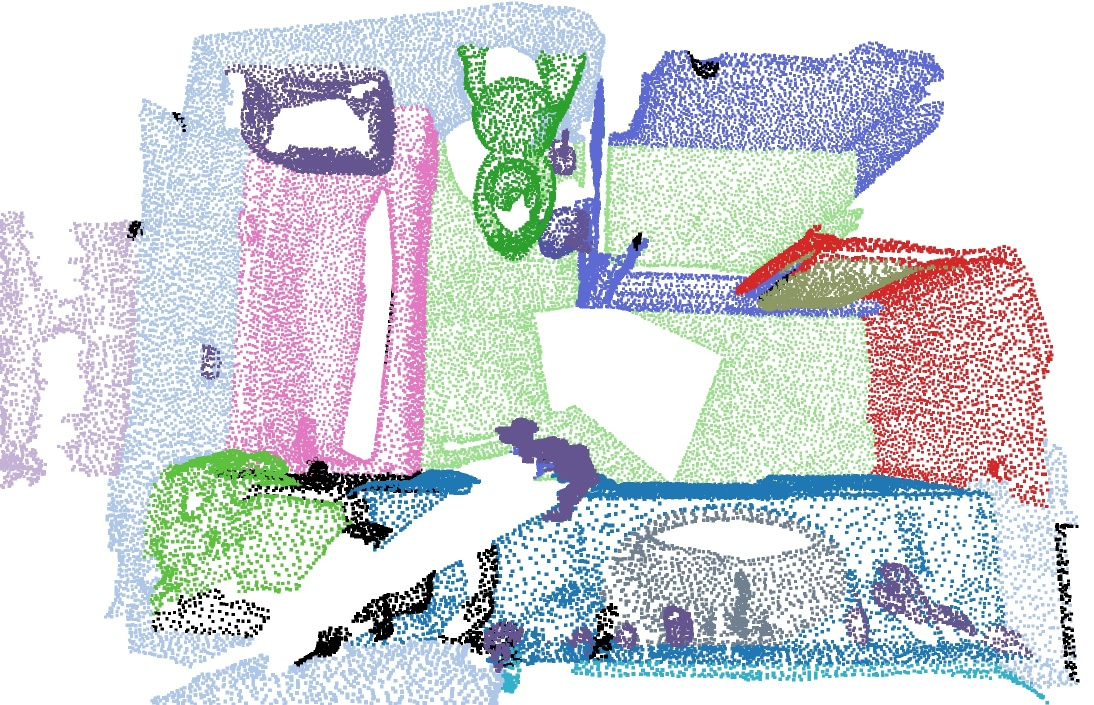
\includegraphics[width=\linewidth]{texturenet/sampling/sampling_fps00.jpg}
    (a) Furthest Point Sampling
    \end{minipage}
    \begin{minipage}{0.4\linewidth}
    \centering
    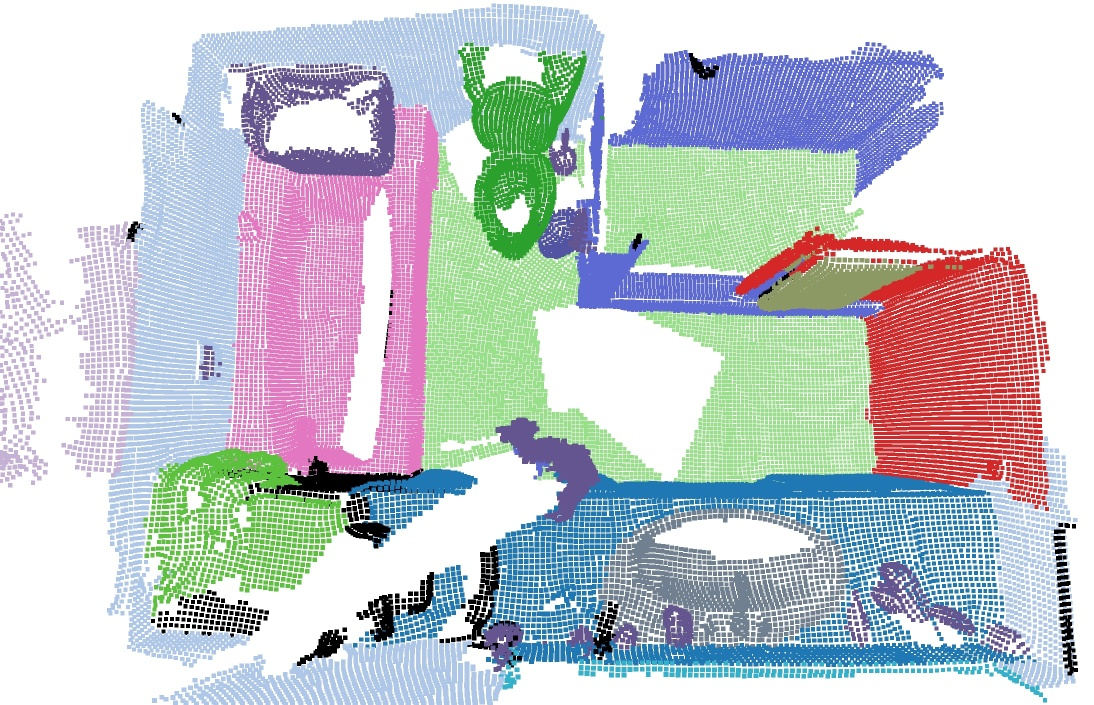
\includegraphics[width=\linewidth]{texturenet/sampling/sampling_ours00.jpg}
    (b) Ours
    \end{minipage}\\
    \vspace{0.1cm}
    \caption{Visualization of Different Sampling methods.}
    \label{fig:texturenet-sampling}
\end{figure}

The next experiment tests the impact of our proposed point sampling method.  While PointNet++~\cite{qi2017pointnet++} adopts the furthest point sampling method to preprocess the data, we use QuadriFlow~\cite{huang2018quadriflow} to sample the points on the surface. It maintains uniform edge length in surface parametrization, and therefore usually provides more uniformly distributed samples on the surface considering the geodesic distance. Figure~\ref{fig:texturenet-sampling} shows the proportion of each class in the ScanNet dataset with QuadriFlow and furthest point sampling.

We use TextureNet to learn the semantic labels with their input and our samples. Table~\ref{tab:texturenet-sample} shows the  class IoU for the prediction. With more samples for minor classes like the counter, desk, and curtain, our sampling method performs better. Figure~\ref{fig:texturenet-sampling} shows the visualization of different sampling results. Visually, our sampling method leads to more uniformly distributed points on the surface.

\begin{figure}[h]
    \centering
    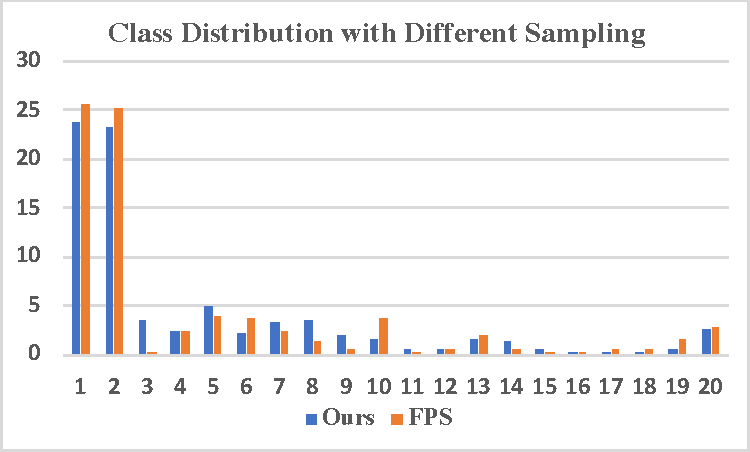
\includegraphics[width=0.6\linewidth]{texturenet/diagram/class.pdf}
    \caption{Class distribution with different sampling. The y-axis represents the portion of each class across all scenes. Except for classes of wall, floor, and bookshelf, our method achieves more samples than the furthest sampling method. As a result, PointNet++ achieves better results in most classes with our sampling method.}
    \label{fig:texturenet-sampling-vis}
\end{figure}




%%%%%%%%%%%%%%%%%%%%%%%%%%%%%%%%%%%%%%%%%%%%%%%%%%%%%%%%
\section{Further Results on Effect of 4-RoSy Surface Convolution}
\label{appendix:4rosy}
Table~\ref{tab:texturenet-appendix-operator} provides detailed results for the performance of different surface convolution operators on ScanNet dataset~\cite{dai2017scannet} with input as the point cloud or the point cloud associated with the normal and RGB color for each point (expanding on Table 4 of the paper).    
PN$^+$(A) and PN$^+$ represent PointNet++ with average-pooling and maxpooling, respectively. GCNN$^1$ and GCNN are geodesic convolutional neural networks~\cite{masci2015geodesic} with $N_\rho=3,N_\theta=1$ and $N_\rho=N_\theta=3$ respectively. 
ACNN represents anisotropic convolutional neural networks~\cite{boscaini2016learning} with $N_\rho=3=N_\theta=3$. RoSy$^1$ refers to a 3x3 convolution along the direction of the 1-rosy orientation field. 
RoSy$^4$ picks an arbitrary direction from the cross in the 4-rosy field. RoSy$^4$(m) applies 3x3 convolution for each direction of the cross in the 4-rosy field, aggregated by max pooling. 
Ours(A) and Ours represent our method with average-pooling and max-pooling aggregation.
\begin{table*}
    \centering
    \scriptsize
    \tabcolsep=0.04cm
    \begin{tabular}{|c|c|c|c|c|c|c|c|c|c|c|c|c|c|c|c|c|c|c|c|c|c|}
        \hline
         Operator & wall & floor & cab & bed & chair & sofa & table & door & wind & bkshf & pic & cntr & desk & curt & fridg & show & toil & sink & bath & other & ave\\
        \hline
         PN$^+$(A) & 55.7 & 80.2 & 23.1 & 41.6 & 54.1 & 55.9 & \textbf{68.6} & 11.2 & 20.0 & 41.1 & 5.3 & 37.5 & 36.2 & 4.7 & 2.9 & 6.0 & 30.6 & 21.9 & 48.1 & 7.8 & 32.6\\
         \hline
         PN$^+$ & \textbf{68.7} & 89.9 & 38.3 & 60.1 & 73.5 & 62.0 & 62.2 & 30.9 & 28.2 & 52.8 & 9.6 & 42.7 & 38.6 & 38.4 & 23.4 & 35.7 & 66.2 & 47.6 & 57.4 & 26.0 & 47.6\\
        \hline
         GCNN$^1$ & 62.5 & 94.0 & 35.8 & 65.6 & 73.2 & 63.9 & 59.5 & 30.0 & 32.0 & 57.6 & 11.6 & 53.0 & 38.9 & 40.6 & 29.7 & 46.0 & 59.8 & 43.8 & 48.9 & 27.5 & 48.7\\
        \hline
         GCNN & 54.4 & 81.8 & 17.4 & 9.9 & 48.1 & 24.2 & 28.2 & 16.0 & 24.5 & 15.5 & 9.5 & 18.8 & 15.1 & 27.7 & 6.3 & 20.3 & 27.7 & 23.0 & 9.1 & 13.5 & 24.6 \\
        \hline
         ACNN & 65.1 & 88.0 & 17.0 & 23.0 & 54.2 & 18.7 & 35.9 & 16.4 & 28.1 & 0.3 & \textbf{14.6} & 22.0 & 23.4 & 25.6 & 7.0 & 23.1 & 43.6 & 36.9 & 33.6 & 17.5 & 29.7 \\
        \hline
         RoSy$^1$ & 49.4 & 80.5 & 24.5 & 41.3 & 65.7 & 48.8 & 39.1 & 19.3 & 28.2 & 44.7 & 8.6 & 36.1 & 25.2 & 30.9 & 16.7 & 38.9 & 52.9 & 37.8 & 47.3 & 19.4 & 37.8 \\
         \hline
         RoSy$^4$ & 55.4 & 90.8 & 25.3 & 24.5 & 56.0 & 29.5 & 43.0 & 16.9 & 19.9 & 29.7 & 6.0 & 21.6 & 17.3 & 32.7 & 9.0 & 33.0 & 29.7 & 21.1 & 34.2 & 20.5 & 30.9 \\
         \hline
         RoSy$^4$(m) & 61.3 & 88.2 & 26.7 & 47.6 & \textbf{80.6} & 50.5 & 52.1 & 12.7 & 31.5 & 46.1 & 13.7 & 47.4 & 25.1 & 20.9 & 9.8 & 29.8 & 50.2 & 41.1 & 43.6 & 27.7 & 40.3 \\
         \hline
         Ours(A) & 51.5 & 87.1 & 26.0 & 44.7 & 65.0 & 46.4 & 42.5 & 18.5 & 31.4 & 29.0 & 8.0 & 40.6 & 24.9 & 11.5 & 18.9 & 34.9 & 61.2 & 43.0 & 50.2 & 23.8 & 38.0\\
        \hline
         Ours & 64.8 & \textbf{90.0} & \textbf{39.3} & \textbf{65.8} & 74.8 & \textbf{66.6} & 50.5 & \textbf{33.9} & \textbf{35.6} & \textbf{58.0} & 14.0 & \textbf{54.3} & \textbf{42.1} & \textbf{45.4} & \textbf{30.9} & \textbf{43.0} & \textbf{67.7} & \textbf{47.9} & \textbf{55.8} & \textbf{32.2} & \textbf{50.6} \\
        \hline
    \end{tabular}\\
    (a) Pointcloud\\
    \centering
    \tabcolsep=0.04cm
    \begin{tabular}{|c|c|c|c|c|c|c|c|c|c|c|c|c|c|c|c|c|c|c|c|c|c|}
        \hline
         Operator & wall & floor & cab & bed & chair & sofa & table & door & wind & bkshf & pic & cntr & desk & curt & fridg & show & toil & sink & bath & other & ave\\
        \hline
         PN$^+$(A) & 66.6 & 94.7 & 29.9 & 50.5 & 64.9 & 52.9 & 56.5 & 17.4 & 19.7 & 45.0 & 0.0 & 36.5 & 30.4 & 21.5 & 13.5 & 19.1 & 49.6 & 30.3 & 45.6 & 16.6 & 38.1\\
         \hline
         PN$^+$~\cite{qi2017pointnet++} & \textbf{81.5} & \textbf{95.0} & 40.1 & 60.0 & 74.9 & 52.8 & 46.1 & 31.3 & 19.7 & 50.3 & 5.9 & 33.9 & 25.9 & \textbf{58.2} & 30.0 & \textbf{48.6} & \textbf{85.2} & 47.1 & 48.8 & 28.5 & 48.2\\
        \hline
         GCNN$^1$ & 69.4 & 93.1 & 37.3 & 65.4 & 68.6 & 54.3 & \textbf{59.0} & 35.7 & 34.6 & 56.7 & 17.5 & 51.8 & 40.2 & 39.6 & 27.0 & 47.0 & 57.7 & 39.9 & \textbf{69.4} & 28.6 & 49.6 \\
        \hline
         GCNN~\cite{masci2015geodesic} & 46.8 & 89.1 & 21.1 & 31.5 & 52.1 & 36.6 & 41.6 & 17.2 & 18.1 & 21.3 & 3.7 & 23.5 & 17.7 & 22.6 & 4.9 & 16.7 & 24.6 & 22.7 & 16.9 & 11.3 & 27.0 \\
        \hline
         ACNN~\cite{boscaini2016anisotropic} & 58.4 & 89.2 & 23.8 & 30.6 & 61.5 & 29.7 & 39.4 & 18.5 & 25.4 & 14.2 & 5.1 & 33.7 & 19.2 & 29.0 & 8.6 & 30.7 & 41.6 & 35.5 & 36.4 & 17.0 & 32.4 \\
        \hline
         RoSy$^1$ & 56.3 & 90.9 & 34.9 & 50.5 & 73.5 & 58.6 & 51.7 & 30.7 & 39.9 & 56.1 & 9.7 & 45.1 & 36.7 & 39.5 & 28.2 & 42.8 & 68.6 & 49.5 & 64.6 & 29.3 & 47.8 \\
         \hline
         RoSy$^4$ & 51.7 & 89.3 & 26.0 & 39.1 & 60.8 & 37.4 & 42.8 & 10.4 & 30.6 & 39.1 & 14.9 & 35.9 & 19.7 & 17.4 & 8.6 & 21.0 & 42.3 & 38.0 & 36.4 & 19.6 & 34.5 \\
         \hline
         RoSy$^4$(m) & 66.2 & 93.4 & 33.7 & 50.3 & \textbf{78.5} & 47.6 & 54.9 & 13.4 & 39.0 & 49.7 & \textbf{18.8} & 46.5 & 24.9 & 22.2 & 10.7 & 27.2 & 54.2 & 48.8 & 46.5 & 25.4 & 42.6 \\
         \hline
         Ours(A) & 52.4 & 91.3 & 29.1 & 42.5 & 65.6 & 42.1 & 47.3 & 20.6 & 31.4 & 30.9 & 7.3 & 40.8 & 26.2 & 10.7 & 18.2 & 31.2 & 64.8 & 44.1 & 63.6 & 21.1 & 39.1 \\
        \hline
         Ours & 69.8 & 92.3 & \textbf{44.8} & \textbf{69.4} & 75.8 & \textbf{67.1} & 56.8 & \textbf{39.4} & \textbf{41.1} & \textbf{63.1} & 15.8 & \textbf{57.4} & \textbf{46.5} & 48.3 & \textbf{36.9} & 40.0 & 78.1 & \textbf{54.0} & 65.4 & \textbf{34.4} & \textbf{54.8} \\
        \hline
    \end{tabular}\\
    (b) Pointcloud with per-point normal and RGB color\\
    \caption{Texture Convolution Operator Comparison. The input is the pointcloud in (a) and the pointcloud associated with the normal and the rgb color for each point in (b). PN$^+$(A) and PN$^+$ represent PointNet++ with average-pooling and maxpooling, respectively. GCNN$^1$ and GCNN are geodesic convolutional neural networks~\cite{masci2015geodesic} with $N_\rho=3,N_\theta=1$ and $N_\rho=N_\theta=3$ respectively. ACNN represents anisotropic convolutional neural networks~\cite{boscaini2016learning} with $N_\rho=3,N_\theta=1$. RoSy$^1$ means a 3x3 convolution along the direction of the 1-rosy orientation field. RoSy$^4$ picks an arbitrary direction from the cross in the 4-rosy field. RoSy$^4$(m) applies 3x3 convolution for each direction of the cross in the 4-rosy field, aggregated by maxpooling. Ours(A) and Ours represent our method with average-pooling and max-pooling aggregation.}
    \label{tab:texturenet-appendix-operator}
\end{table*}

\section{Comparison to Octree-based Approaches} 
\label{appendix:ocnn}
\jw{Existing volume-based octree methods have been used mostly for stand-alone objects from ShapeNet.
For larger scenes, memory is a severe limitation.
As a test, we tried O-CNN~\cite{wang2017cnn} on chunks of radius 1.35m$^3$ using a 12GB GPU, which fits 6 conv/deconv layers and a feature dimension of 256 at resolution $256^3$.  This test yielded a mean IoU of 30.8 with NRGB and 27.8 with pure geometry. 
In contrast, the surface-based convolution of TextureNet is much more efficient (2D rather than 3D), allowing for a total of 18 conv/deconv layers with max feature dimension of 1024, and achieves 58.1 with high-res color, 54.8 with NRGB, and 50.6 with pure geometry.  }

\vspace{-0.1in}
%%%%%%%%%%%%%%%%%%%%%%%%%%%%%%%%%%%%%%%%%%
\section{Further Comparisons Using Only Surface Geometry}
\label{appendix:geometry}
This section provides more detailed results for the experiment described in the last paragraph of Section 4 of the paper, where we evaluate the value of the proposed 3D network for semantic segmentation of inputs with only surface geometry (without color).  During experiments on ScanNet, TextureNet achieves 50.6\% mIoU, which is 6.4\% better than the previous state-of-the-art.   In comparison, ScanNet~\cite{dai2017scannet} = 30.6\%, Tangent Convolution~\cite{tatarchenko2018tangent} = 40.9\%, PointNet++~\cite{qi2017pointnet++} = 43.5\%, and SplatNet~\cite{su2018splatnet} = 44.2\%.  Detailed class IoU results are provided in Table~\ref{tab:texturenet-geometry}.

\begin{table*}
    \centering
    \scriptsize
    \tabcolsep=0.03cm
    \begin{tabular}{|c|c|c|c|c|c|c|c|c|c|c|c|c|c|c|c|c|c|c|c|c|c|}
        \hline
        Input & wall & floor & cab & bed & chair & sofa & table & door & wind & shf & pic & cntr & desk & curt & fridg & show & toil & sink & bath & other & avg\\
        \hline
        ScanNet~\cite{dai2017scannet} & 43.7 & 78.6 & 31.1 & 36.6 & 52.4 & 34.8 & 30.0 & 18.9 & 18.2 & 50.1 & 10.2 & 21.1 & 34.2 & 0.0 & 24.5 & 15.2 & 46.0 & 31.8 & 20.3 & 14.5 & 30.6\\
        \hline
        PN$^+$~\cite{qi2017pointnet++} & 64.1 & 82.2 & 31.4 & 51.6 & 64.5 & 51.4 & 44.9 & 23.3 & 30.4 & \textbf{68.2} & 3.7 & 26.2 & 34.2 & \textbf{65.1} & 23.4 & 18.3 & 61.8 & 31.5 & \textbf{75.4} & 18.8 & 43.5\\
        \hline
        SplatNet~\cite{su2018splatnet} & \textbf{67.4} & 85.8 & 32.3 & 45.1 & 71.9 & 51.0 & 40.7 & 15.1 & 25.2 & 62.3 & 0.0 & 23.2 & 39.9 & 56.1 & 0.0 & 24.2 & 62.6 & 23 & 67.4 & 25.7 & 40.9\\
        \hline
        Tangent~\cite{tatarchenko2018tangent} & 62.0 & 83.6 & 39.3 & 58.4 & 67.6 & 57.3 & 47.9 & 27.6 & 28.5 & 55.0 & 8.3 & 36.1 & 33.9 & 38.7 & 26.2 & 28.0 & 60.5 & 39.3 & 59.0 & 27.8 & 44.2\\
        \hline
        Ours & 64.8 & \textbf{90.0} & \textbf{39.3} & \textbf{65.8} & \textbf{74.8} & \textbf{66.6} & \textbf{50.5} & \textbf{33.9} & \textbf{35.6} & 58.0 & \textbf{14.0} & \textbf{54.3} & \textbf{42.1} & 45.4 & \textbf{30.9} & \textbf{43.0} & \textbf{67.7} & \textbf{47.9} & 55.8 & \textbf{32.2} & \textbf{50.6}\\
        \hline
    \end{tabular}
    \caption{Geometry-only: comparison to the state-of-the-art for 3D convolution with pure geometry as input; i.e., no RGB information used in any of these experiments. We can show that our method also outperforms existing geometry-only approaches.}
    \label{tab:texturenet-geometry}
\end{table*}

%%%%%%%%%%%%%%%%%%%%%%%%%%%%%%%%%%%%%%%%%%%%%%%%%%%%%%%%
\vspace{-0.1in}
\section{Effect of 4-RoSy convolution on image convolution}

We also compared our 4-RoSy operator with the traditional image convolution on the MNIST dataset~\cite{lecun2010mnist}. We use a simple network containing two MLP layers and two fully connected layers. The performance of the original network is 99.1\%. By replacing the convolution with our 4-RoSy operator in the MLP layers, we achieve 98.5\% classification accuracy. Therefore, our 4-RoSy kernel is comparable to the traditional convolutions even on the standard images.


\vspace{-0.1in}
%%%%%%%%%%%%%%%%%%%%%%%%%%%%%%%%%%%%%%%%%%%%%%%%%%%%%%%%
\section{Visual comparison of Different Resolutions}
In Figure~\ref{fig:texturenet-highres}, we show the predictions of TextureNet with different color resolutions as input. The first column is the 3D model. The second column shows the ground truth semantic labels. The high-res signals of the red regions are shown in the third column. The last two columns are predictions from TextureNet with per-point color (low-res) or high-res texture patch as input. As a result, TextureNet performs better given the input with high-res signals.

\vspace{-0.1in}
%%%%%%%%%%%%%%%%%%%%%%%%%%%%%%%%%%%%%%%%%%%%%%%%%%%%%%%%
\section{Visualization of the Semantic Segmentation}
We compare TextureNet with the state-of-the-art method on ScanNet Dataset~\cite{dai2017scannet} and Matterport3D Dataset. On both datasets, we outperform existing methods (see the main paper). Figure~\ref{fig:texturenet-supple-scannet1} and~\ref{fig:texturenet-supple-scannet2} show examples of prediction from several methods on ScanNet. Figure~\ref{fig:texturenet-supple-matterport} show examples of prediction from different methods on Matterport3D Dataset.

\begin{figure*}
    \centering
    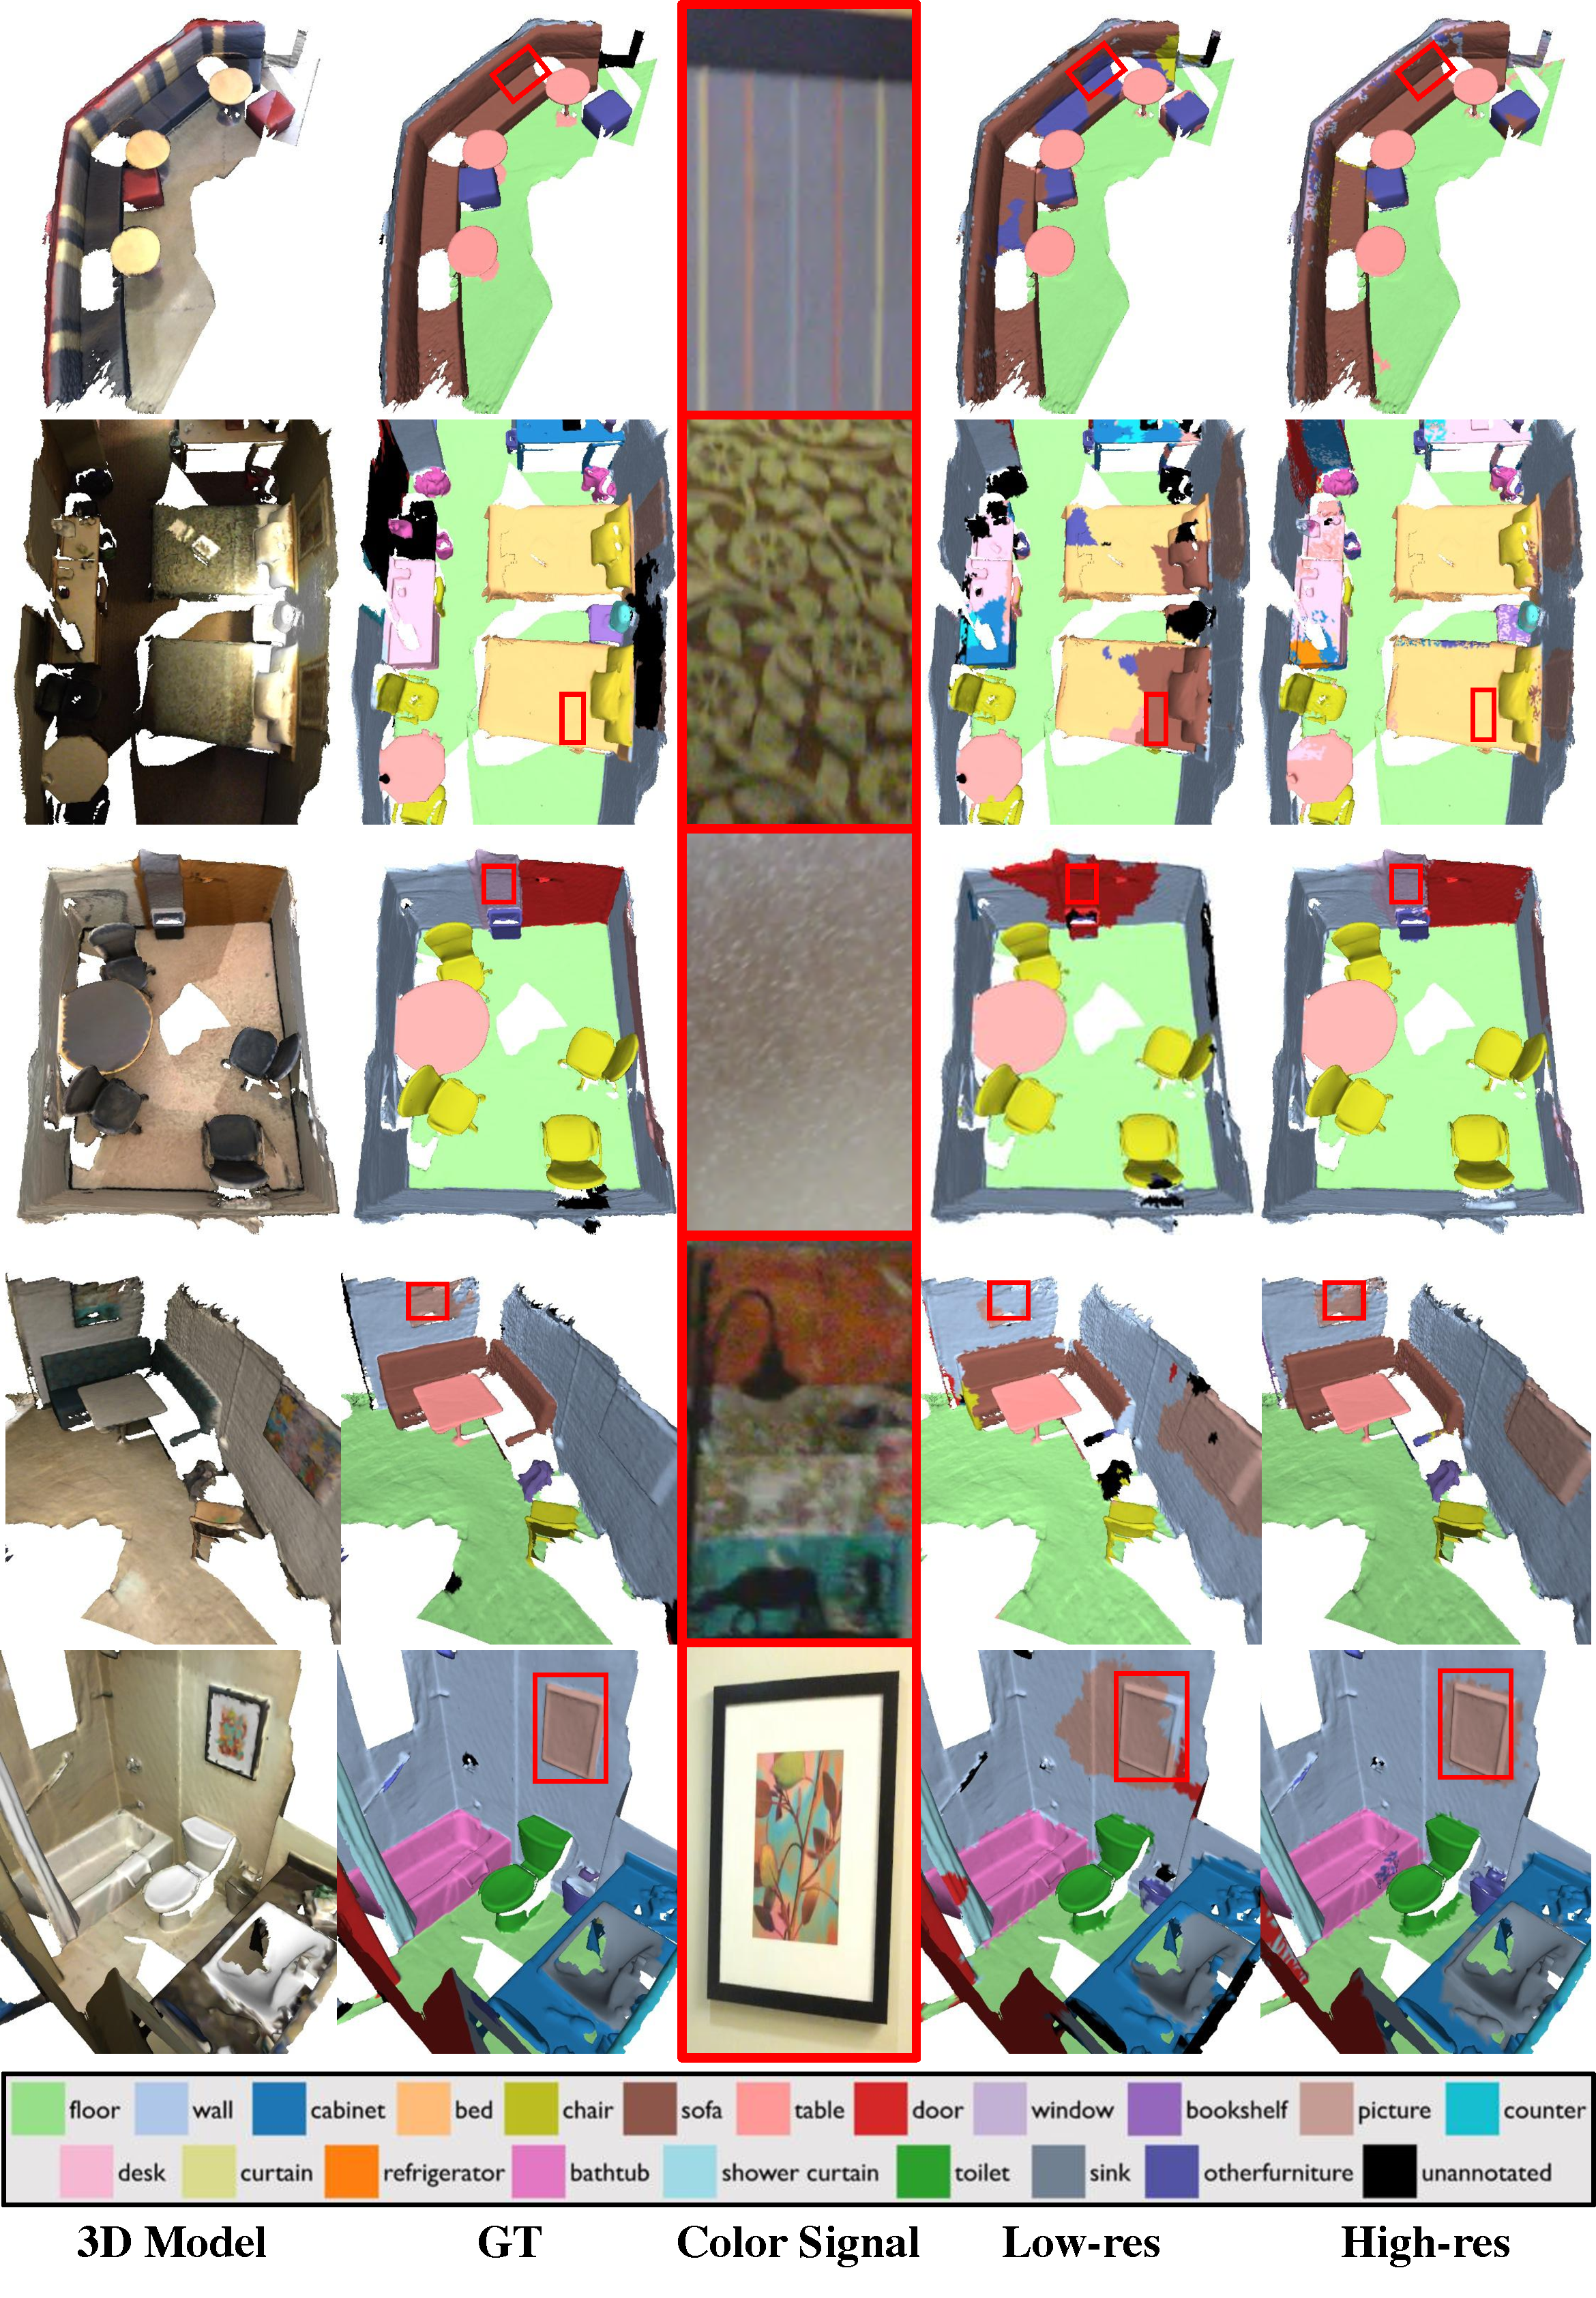
\includegraphics[width=0.75\textwidth]{texturenet/supplemental/highres.pdf}
    \caption{Visual comparison of Different Resolutions. The column row is the 3D model. The second column shows the ground truth semantic labels. The high-res signals of the red regions are shown in the third column. The last two columns are predictions from TextureNet with per-point color (low-res) or high-res texture patch as input.}
    \label{fig:texturenet-highres}
\end{figure*}

\begin{figure*}
\centering
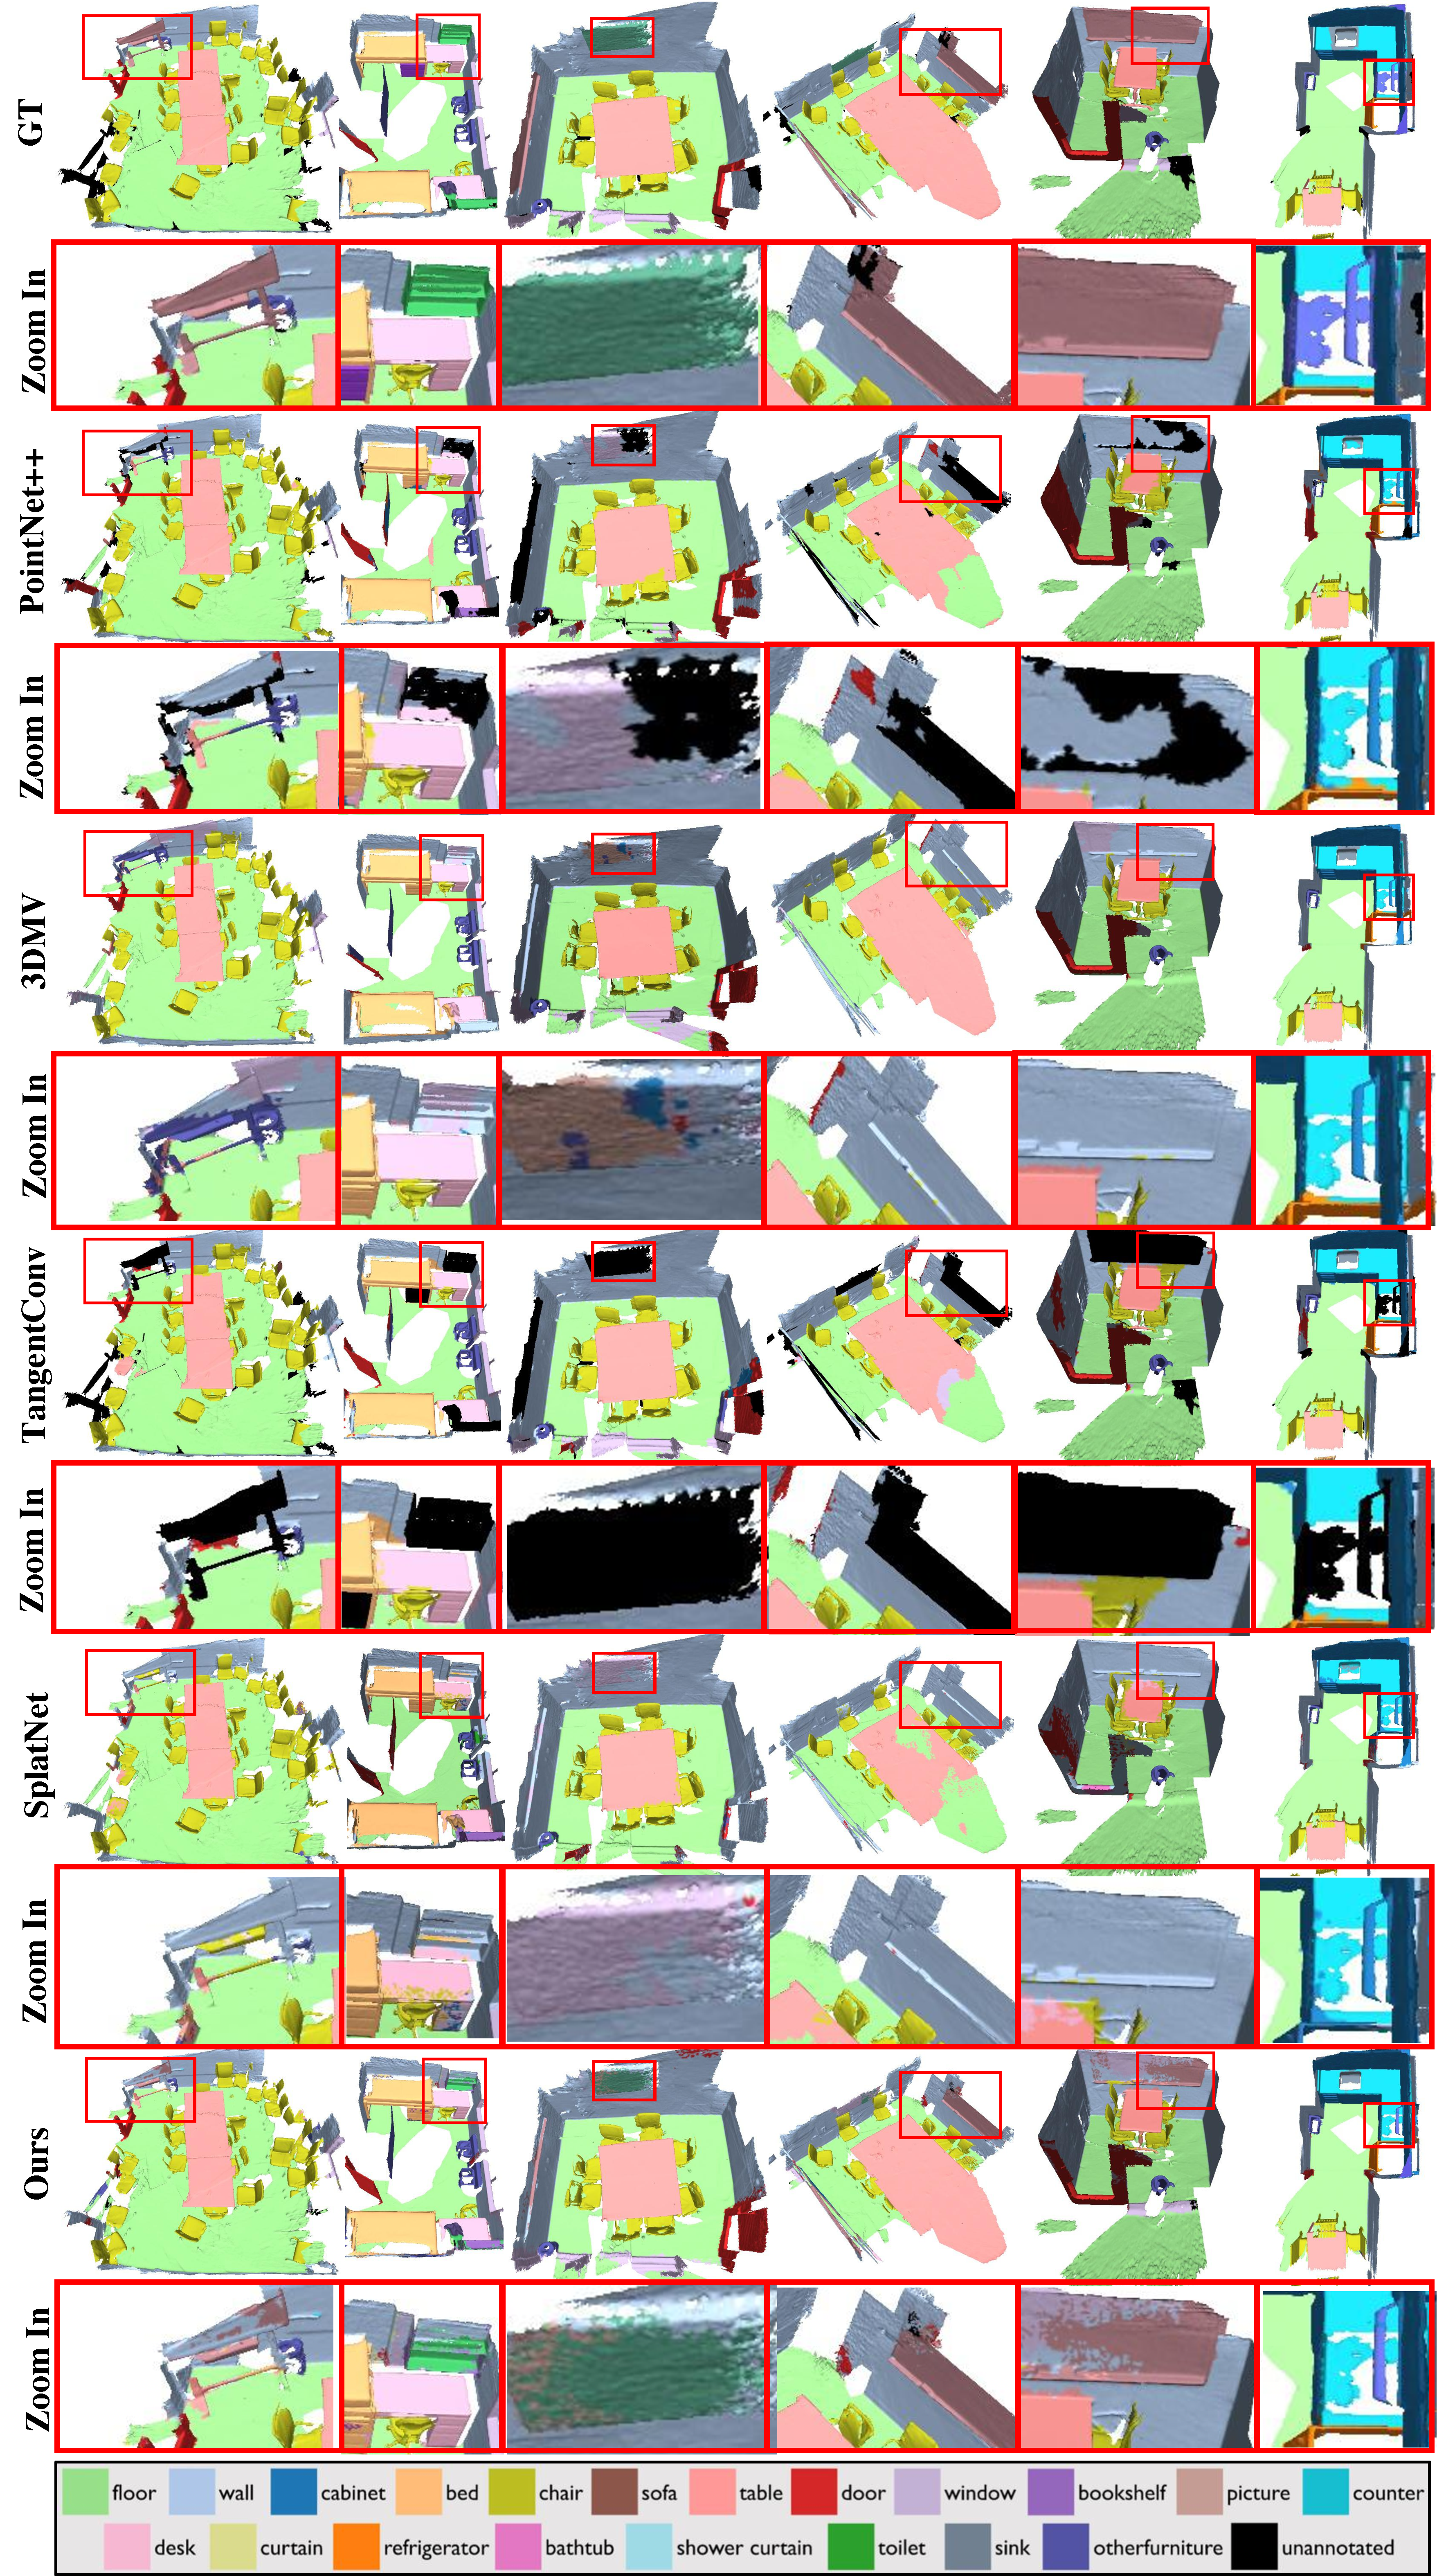
\includegraphics[width=0.7\textwidth]{texturenet/supplemental/supple_scannet1.pdf}
\caption{Visualization of the Semantic Segmentation on ScanNet Dataset.}
\label{fig:texturenet-supple-scannet1}
\end{figure*}

\begin{figure*}
\centering
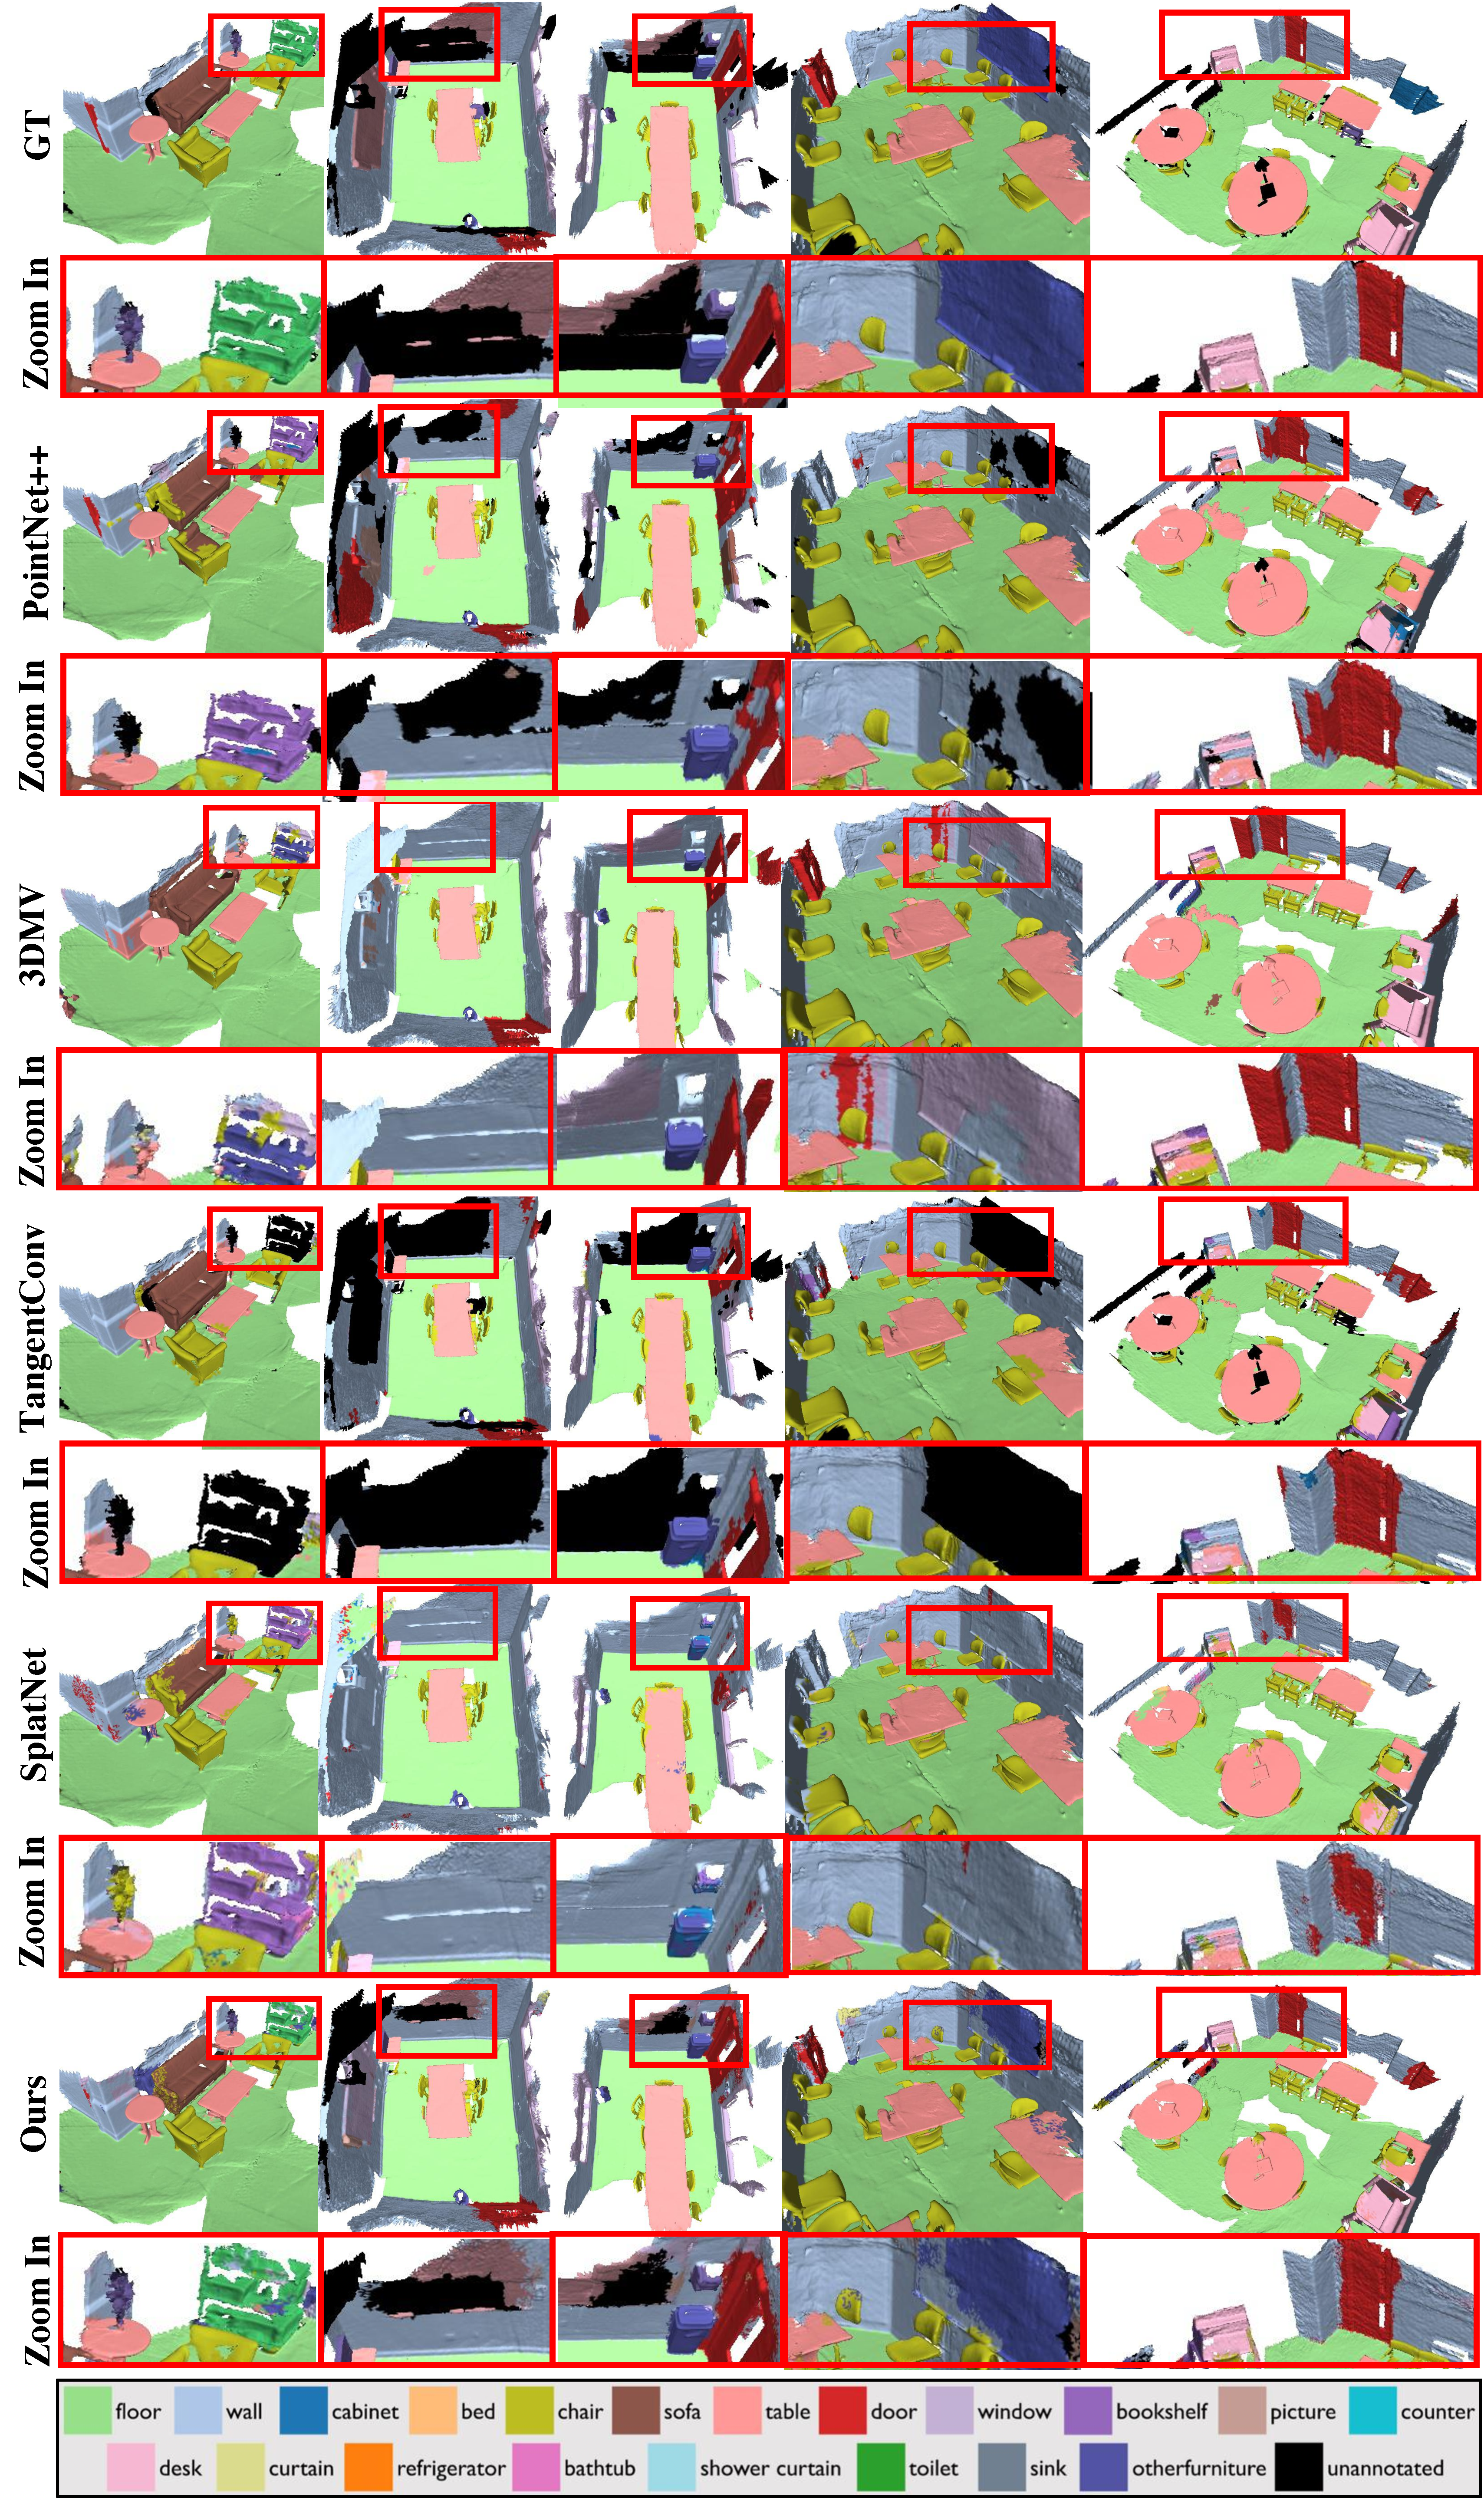
\includegraphics[width=0.7\textwidth]{texturenet/supplemental/supple_scannet2.pdf}
\caption{Visualization of the Semantic Segmentation on ScanNet Dataset.}
\label{fig:texturenet-supple-scannet2}
\end{figure*}

\begin{figure*}
\centering
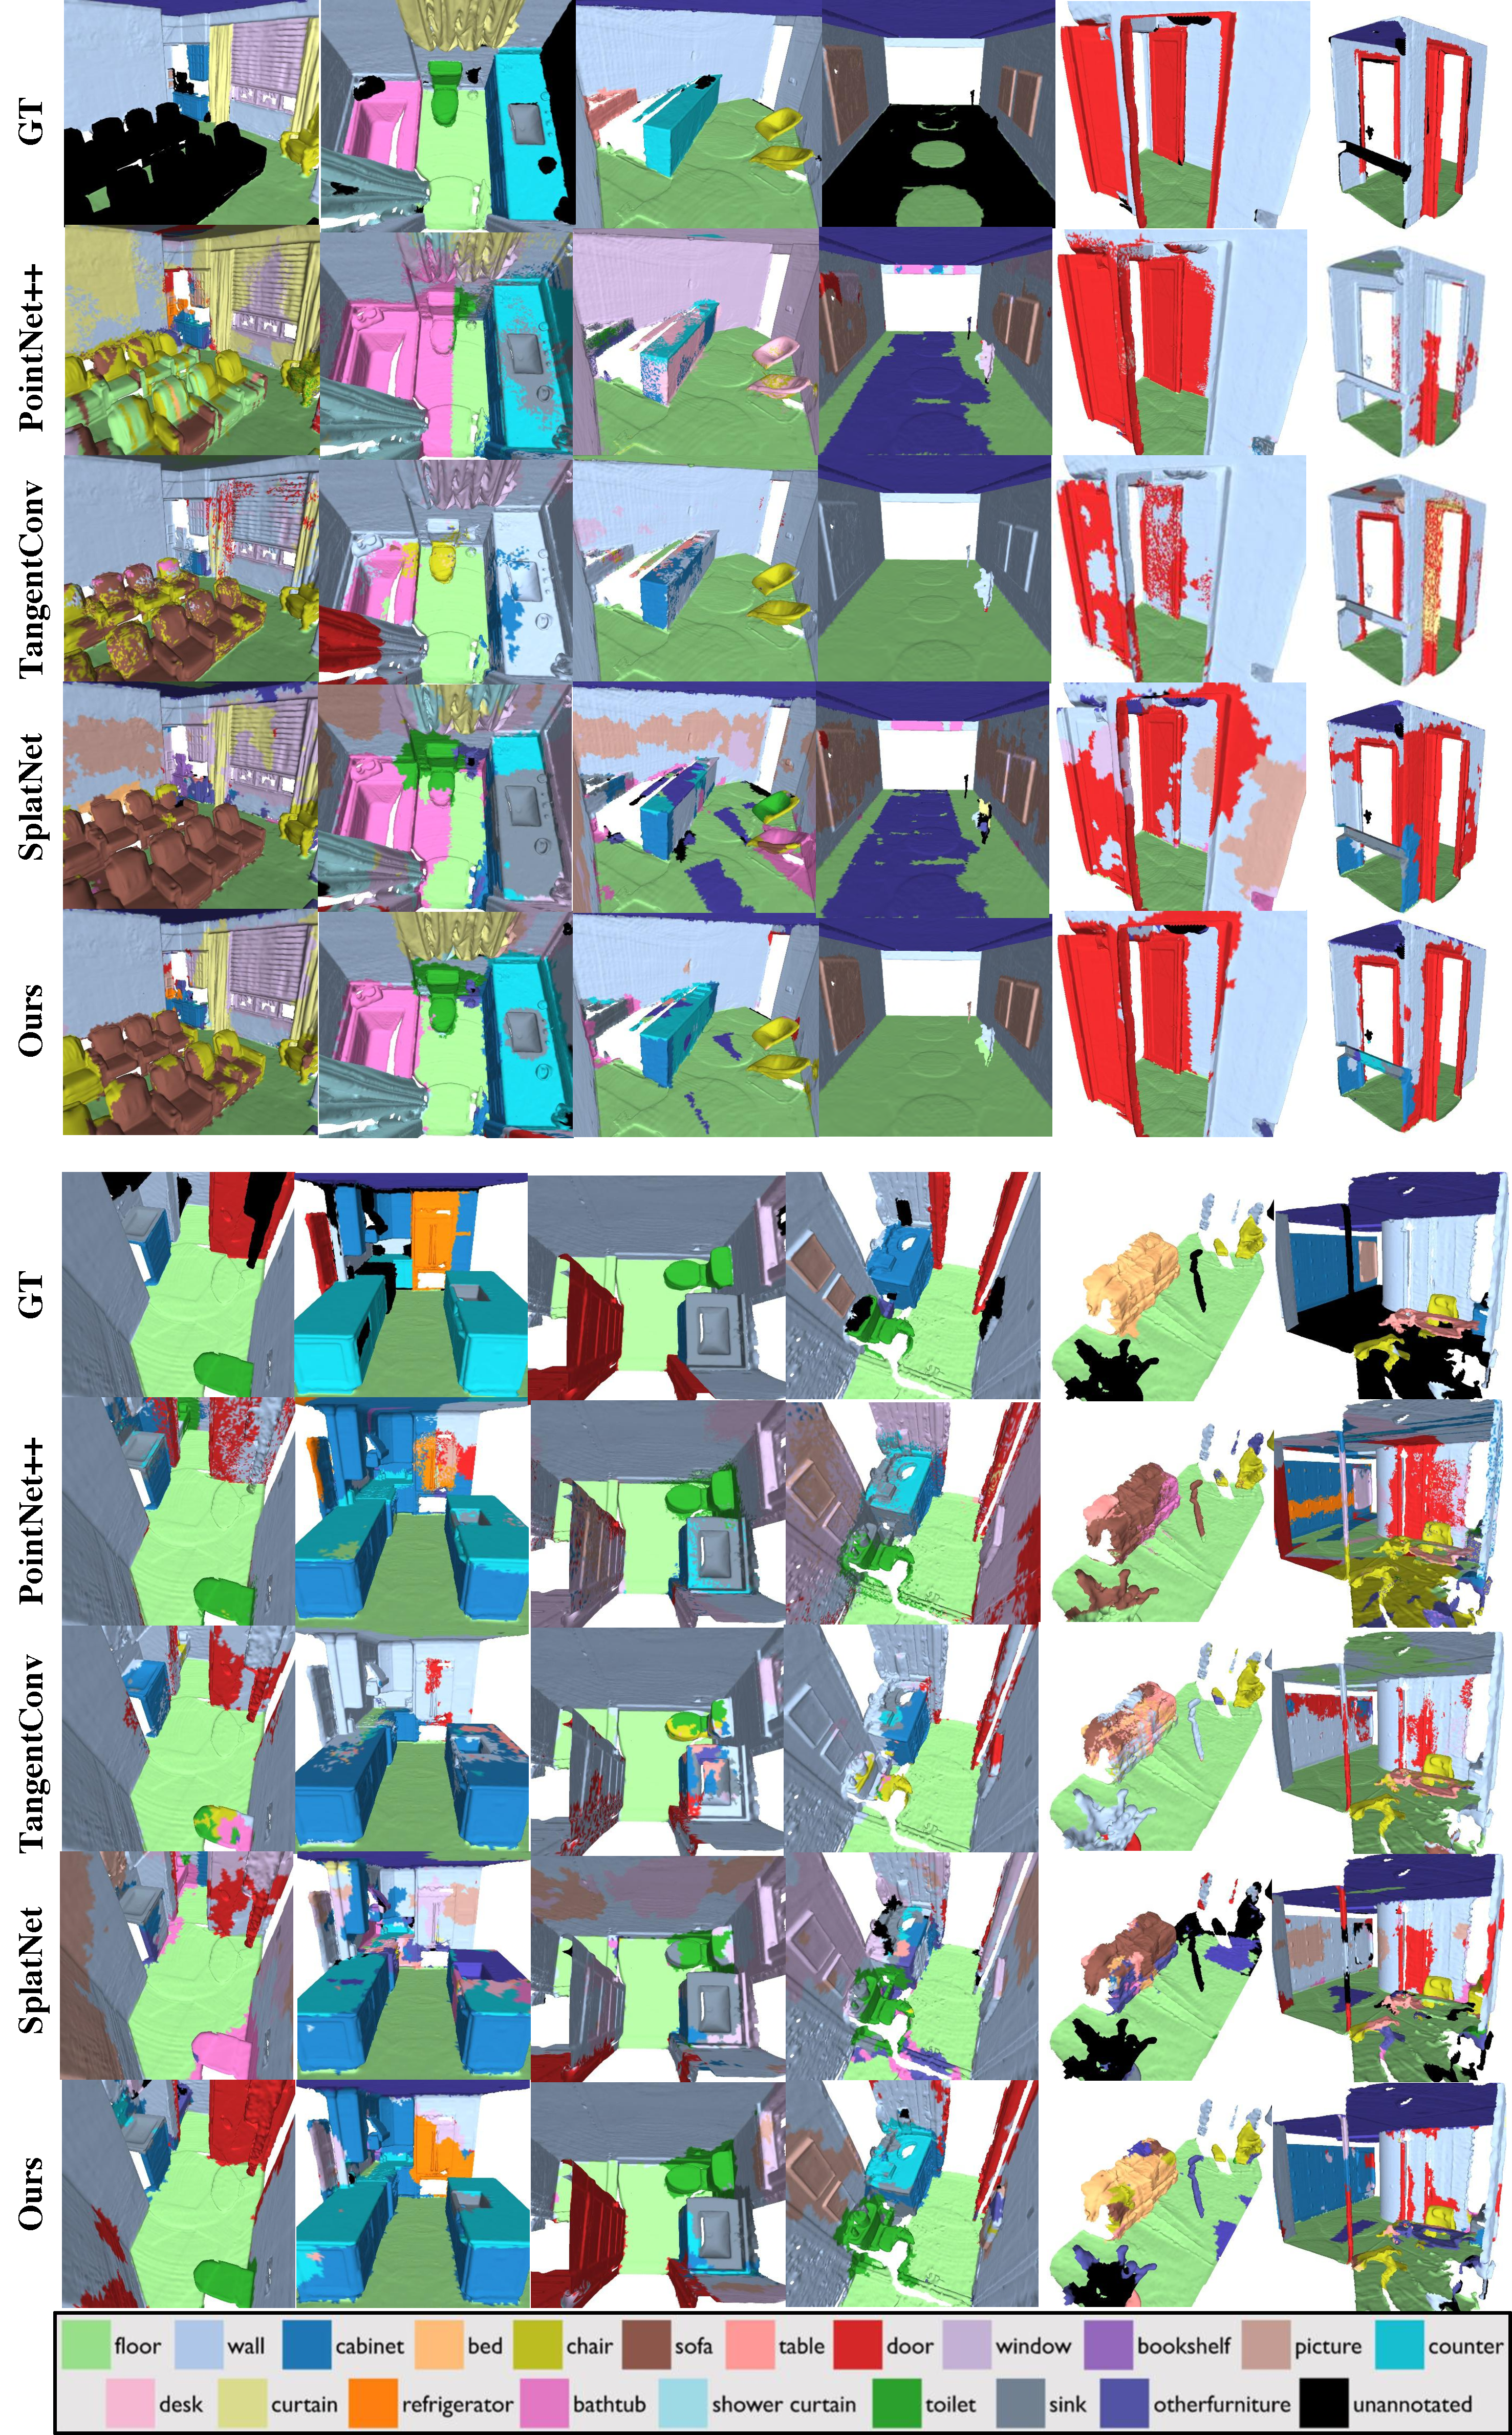
\includegraphics[width=0.7\textwidth]{texturenet/supplemental/supple_matterport.pdf}
\caption{Visualization of the Semantic Segmentation on Matterport Dataset.}
\label{fig:texturenet-supple-matterport}
\end{figure*}

\chapter{More Results on FrameNet}
\section{Implementation Details}
We adopt the original parameters used in DORN~\cite{fu2018deep} for NYUv2 depth estimation, except that we output 13 dimensions at the final layer and use our loss to train the network. During our experiments, the input and output image resolution is 320x240. We use the fixed learning rate as 1e-5.

\section{Additional Baselines}
\paragraph{Necessity to predict both tangent directions and the surface normal}
\cam{We did an experiment on Scannet to test how the results change when only one tangent direction is predicted.  This method yields mean angle errors of $16.34^\circ$ for normals (versus $15.28^\circ$ with ours) and $12.41^\circ$ for tangents (versus $12.26^\circ$ with ours).  Although a normal and one tangent can define a coordinate frame, it is better to predict the second tangent directly rather than deriving it from the normal.  This result corroborates the main thesis of the paper -- predicting tangents helps predicting 3D coordinate frames.}

\paragraph{Geometry prediction followed with canonical frames computation} \cam{We did a baseline experiment where we predict depth and normals using the DORN architecture and then use the resulting surface reconstruction to compute the canonical 3D tangent frame with Quadriflow.  The mean angle error of the tangent directions on the ScanNet test set is $35.84^\circ$, while ours is $12.26^\circ$.  The difference is not surprising since our method is trained with the ground truth tangent supervision.}

\section{Surface Normal Estimation}
\paragraph{Compare with the state-of-the-art} We compare the performance of the surface normal estimation from our approach with the state-of-the-art methods on SunCG~\cite{song2015sun}. We use our approach to train four networks and evaluate them. Table~\ref{tab:scannet-comparison} shows the results including UNet~\cite{ronneberger2015u}, SkipNet~\cite{bansal2016marr}, GeoNet~\cite{qi2018geonet} and DORN~\cite{fu2018deep}. With the assistance of the projected tangent principal directions, the normal prediction has been improved. Please refer to the experiments for ScanNet in the main paper in section 5.1.
\begin{table}[h]
    \centering
    \tabcolsep=0.08cm
    \begin{tabular}{|c|c|c|c||c|c|c|}
        %\hline
         %\textbf{ScanNet} & mean & median & rmse & $11.25^\circ$ & $22.5^\circ$ & $30^\circ$\\
         %\hline
         %UNet & 21.08 & 14.21 & 28.55 & 40.8 & 66.9 & 76.3\\
         %\hline
         %UNet-Ours & 19.68 & 12.43 & 27.58 & 46.1 & 70.6 & 78.8\\
         %\hline
         %SkipNet & 20.36 & 13.74 & 28.63 & 45.4 & 68.2 & 77.4\\
         %\hline
         %SkipNet-Ours & 19.39 & 10.85 & 27.52 & 53.2 & 72.7 & 79.3\\
         %\hline
         %GeoNet & 19.77 & 11.34 & 28.51 & 49.7 & 70.4 & 77.7\\
         %\hline
         %GeoNet-Ours & 18.96 & 9.84 & 27.29 & 54.6 & 73.5 & 80.1\\
         %\hline
         %DORN & 16.42 & 8.64 & 24.94 & 58.7 & 76.7 & 82.9\\
         %\hline
         %DORN-Ours & \textbf{15.28} & \textbf{8.14} & \textbf{23.36} & \textbf{60.6} & \textbf{78.6} & \textbf{84.7}\\
         %\hline         
         %\multicolumn{7}{c}{}\\
         \hline
         \textbf{SunCG} & mean & median & rmse & $11.25^\circ$ & $22.5^\circ$ & $30^\circ$\\
         \hline
         UNet & 14.88 & 6.20 & 24.94 & 64.4 & 78.6 & 83.9\\
         \hline
         UNet-Ours & 13.25 & 4.64 & 23.73 & 69.8 & 81.6 & 86.1\\
         \hline
         SkipNet & 13.38 & 3.97 & 24.54 & 70.2 & 80.3 & 85.1\\
         \hline
         SkipNet-Ours & 12.82 & 3.87 & 23.69 & 71.0 & 80.2 & 86.1\\
         \hline
         GeoNet & 13.14 & 3.56 & 23.54 & 70.6 & 80.7 & 86.0\\
         \hline
         GeoNet-Ours & 12.68 & 3.60 & \textbf{22.73} & 71.2 & 81.3 & \textbf{86.6}\\
         \hline
         DORN & 12.90 & 3.36 & 24.12 & 71.3 & 81.3 & 85.3\\
         \hline
         DORN-Ours & \textbf{12.38} & \textbf{3.33} & 23.34 & \textbf{72.3} & \textbf{82.3} & 86.3\\
         \hline         
    \end{tabular}
    \caption{Evaluation on Surface Normal Predictions. We train and test our algorithm with different network architectures on the SunCG~\cite{dai2017scannet}. Assisted by our joint loss, the performances of all networks are improved.}
    \label{tab:scannet-comparison}
\end{table}

\paragraph{Test on NYUv2} We test different versions of our network on NYUv2~\cite{eigen2014depth} as a standard evaluation dataset. We train the network on SunCG datasets and directly test on NYUv2, as shown in Table~\ref{tab:vis-nyu}. Specifically, GeoNet-origin trained and tested on NYUv2~\cite{qi2018geonet}, and is the current state-of-the-art method on normal estimation. Other rows are networks trained w/o. our joint losses on SunCG.

\begin{table}[h]
    \centering
    \tabcolsep=0.07cm
    \begin{tabular}{|c|c|c|c||c|c|c|}
        \hline
         \textbf{NYUv2} & mean & median & rmse & $11.25^\circ$ & $22.5^\circ$ & $30^\circ$\\
         \hline
         GeoNet-origin & \textbf{19.0} & \textbf{11.8} & \textbf{26.9} & \textbf{48.4} & \textbf{71.5} & \textbf{79.5}\\
         \hline
         \hline
         \textbf{SunCG} & mean & median & rmse & $11.25^\circ$ & $22.5^\circ$ & $30^\circ$\\
         \hline
         UNet & 25.21 & 18.26 & 32.82 & 32.2 & 57.7 & 68.3\\
         \hline
         UNet-Ours & 24.64 & 17.10 & 32.65 & 35.0 & 59.6 & 69.5\\
         \hline
         SkipNet & 24.75 & 17.36 & 32.45 & 33.8 & 58.1 & 69.0\\
         \hline
         SkipNet-Ours & 23.67 & 16.28 & 31.72 & 36.1 & 62.2 & 72.7\\
         \hline
         GeoNet & 22.32 & 14.97 & 30.59 & 39.8 & 64.3 & 73.4\\
         \hline
         GeoNet-Ours & 22.15 & 14.41 & 30.18 & 40.1 & 65.3 & 74.4\\
         \hline
         DORN & 22.19 & 14.46 & 30.16 & 40.3 & 65.3 & 74.1\\
         \hline
         DORN-Ours & 21.99 & 14.29 & 29.87 & 40.5 & 65.8 & 74.6\\
         \hline         
    \end{tabular}
    \caption{Normal prediction on NYUv2~\cite{eigen2014depth}. GeoNet-origin trained and tested on NYUv2~\cite{qi2018geonet}. In other rows, we train network w/o. our joint loss on SunCG and tested on NYUv2. DORN-Ours trained on ScanNet performs best among all.}
    \label{tab:vis-nyu}
\end{table}

The joint loss in the training process results in better normal estimation. From the ScanNet experiment in section 5.1 of the main section,  ScanNet gets better performance compared to SunCG, possibly due to the domain gap between synthetic (SunCG) and real (NYUv2).

\begin{figure}
\begin{minipage}{0.49\linewidth}
    \centering
    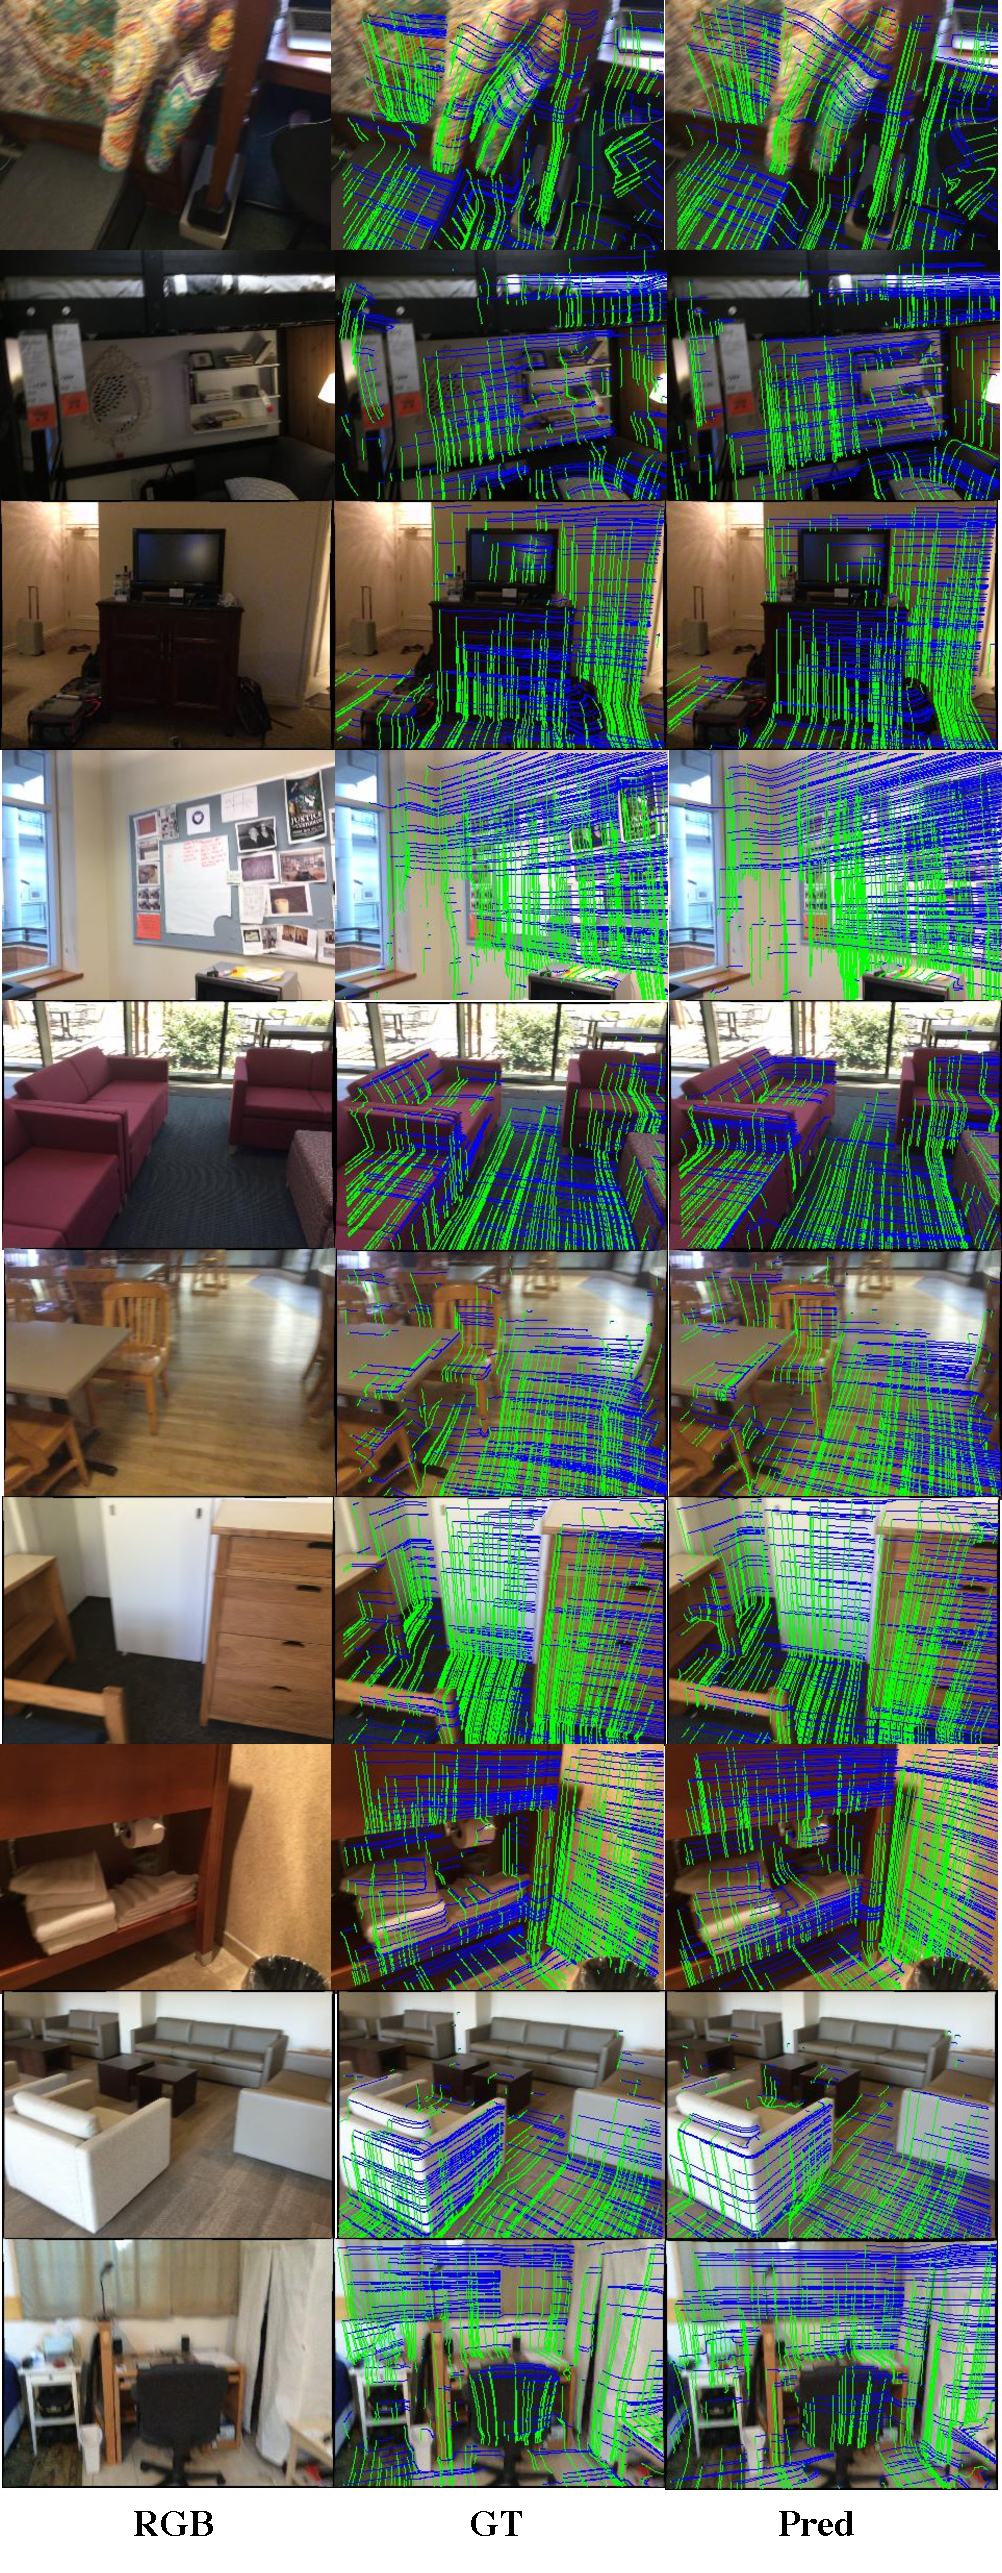
\includegraphics[width=0.95\linewidth]{FrameNet/graph/vis-supplemental.pdf}
    \caption{Visualization of the projected tangent principal directions. The visualization shows similar direction field compared to the ground truth, and is consistent with human intuition.}
    \label{fig:vis-supplemental}
\end{minipage}
\begin{minipage}{0.49\linewidth}
    \centering
    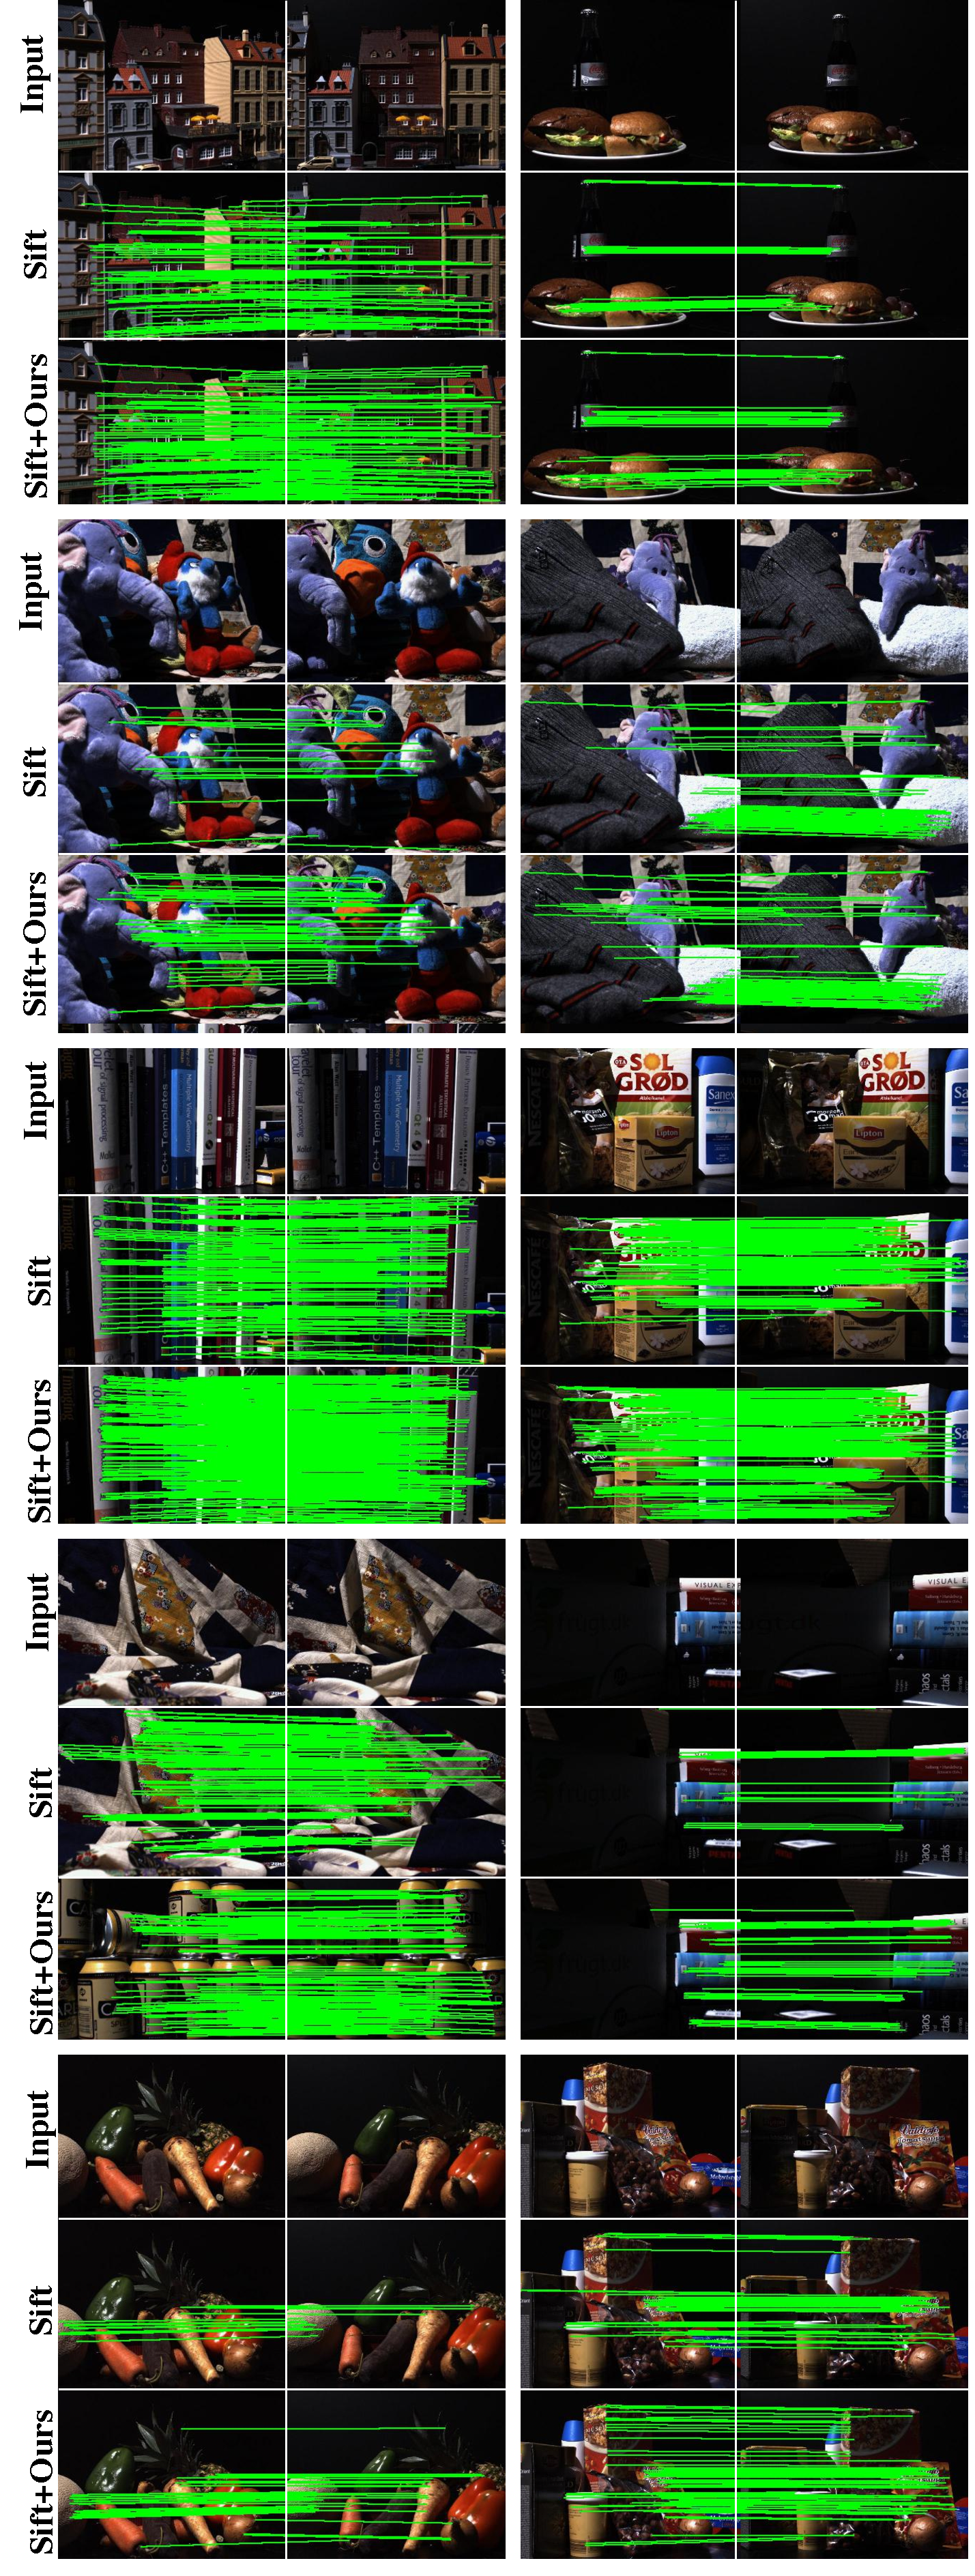
\includegraphics[width=0.92\linewidth]{FrameNet/graph/dtu-supplemental.pdf}
    \caption{Visualization of the feature matching using SIFT and SIFT with our perspective rectification. We produce more correct matching than SIFT does.}
    \label{fig:dtu-supplemental}
\end{minipage}
\end{figure}
\begin{figure}
\begin{minipage}{0.49\linewidth}
    \centering
    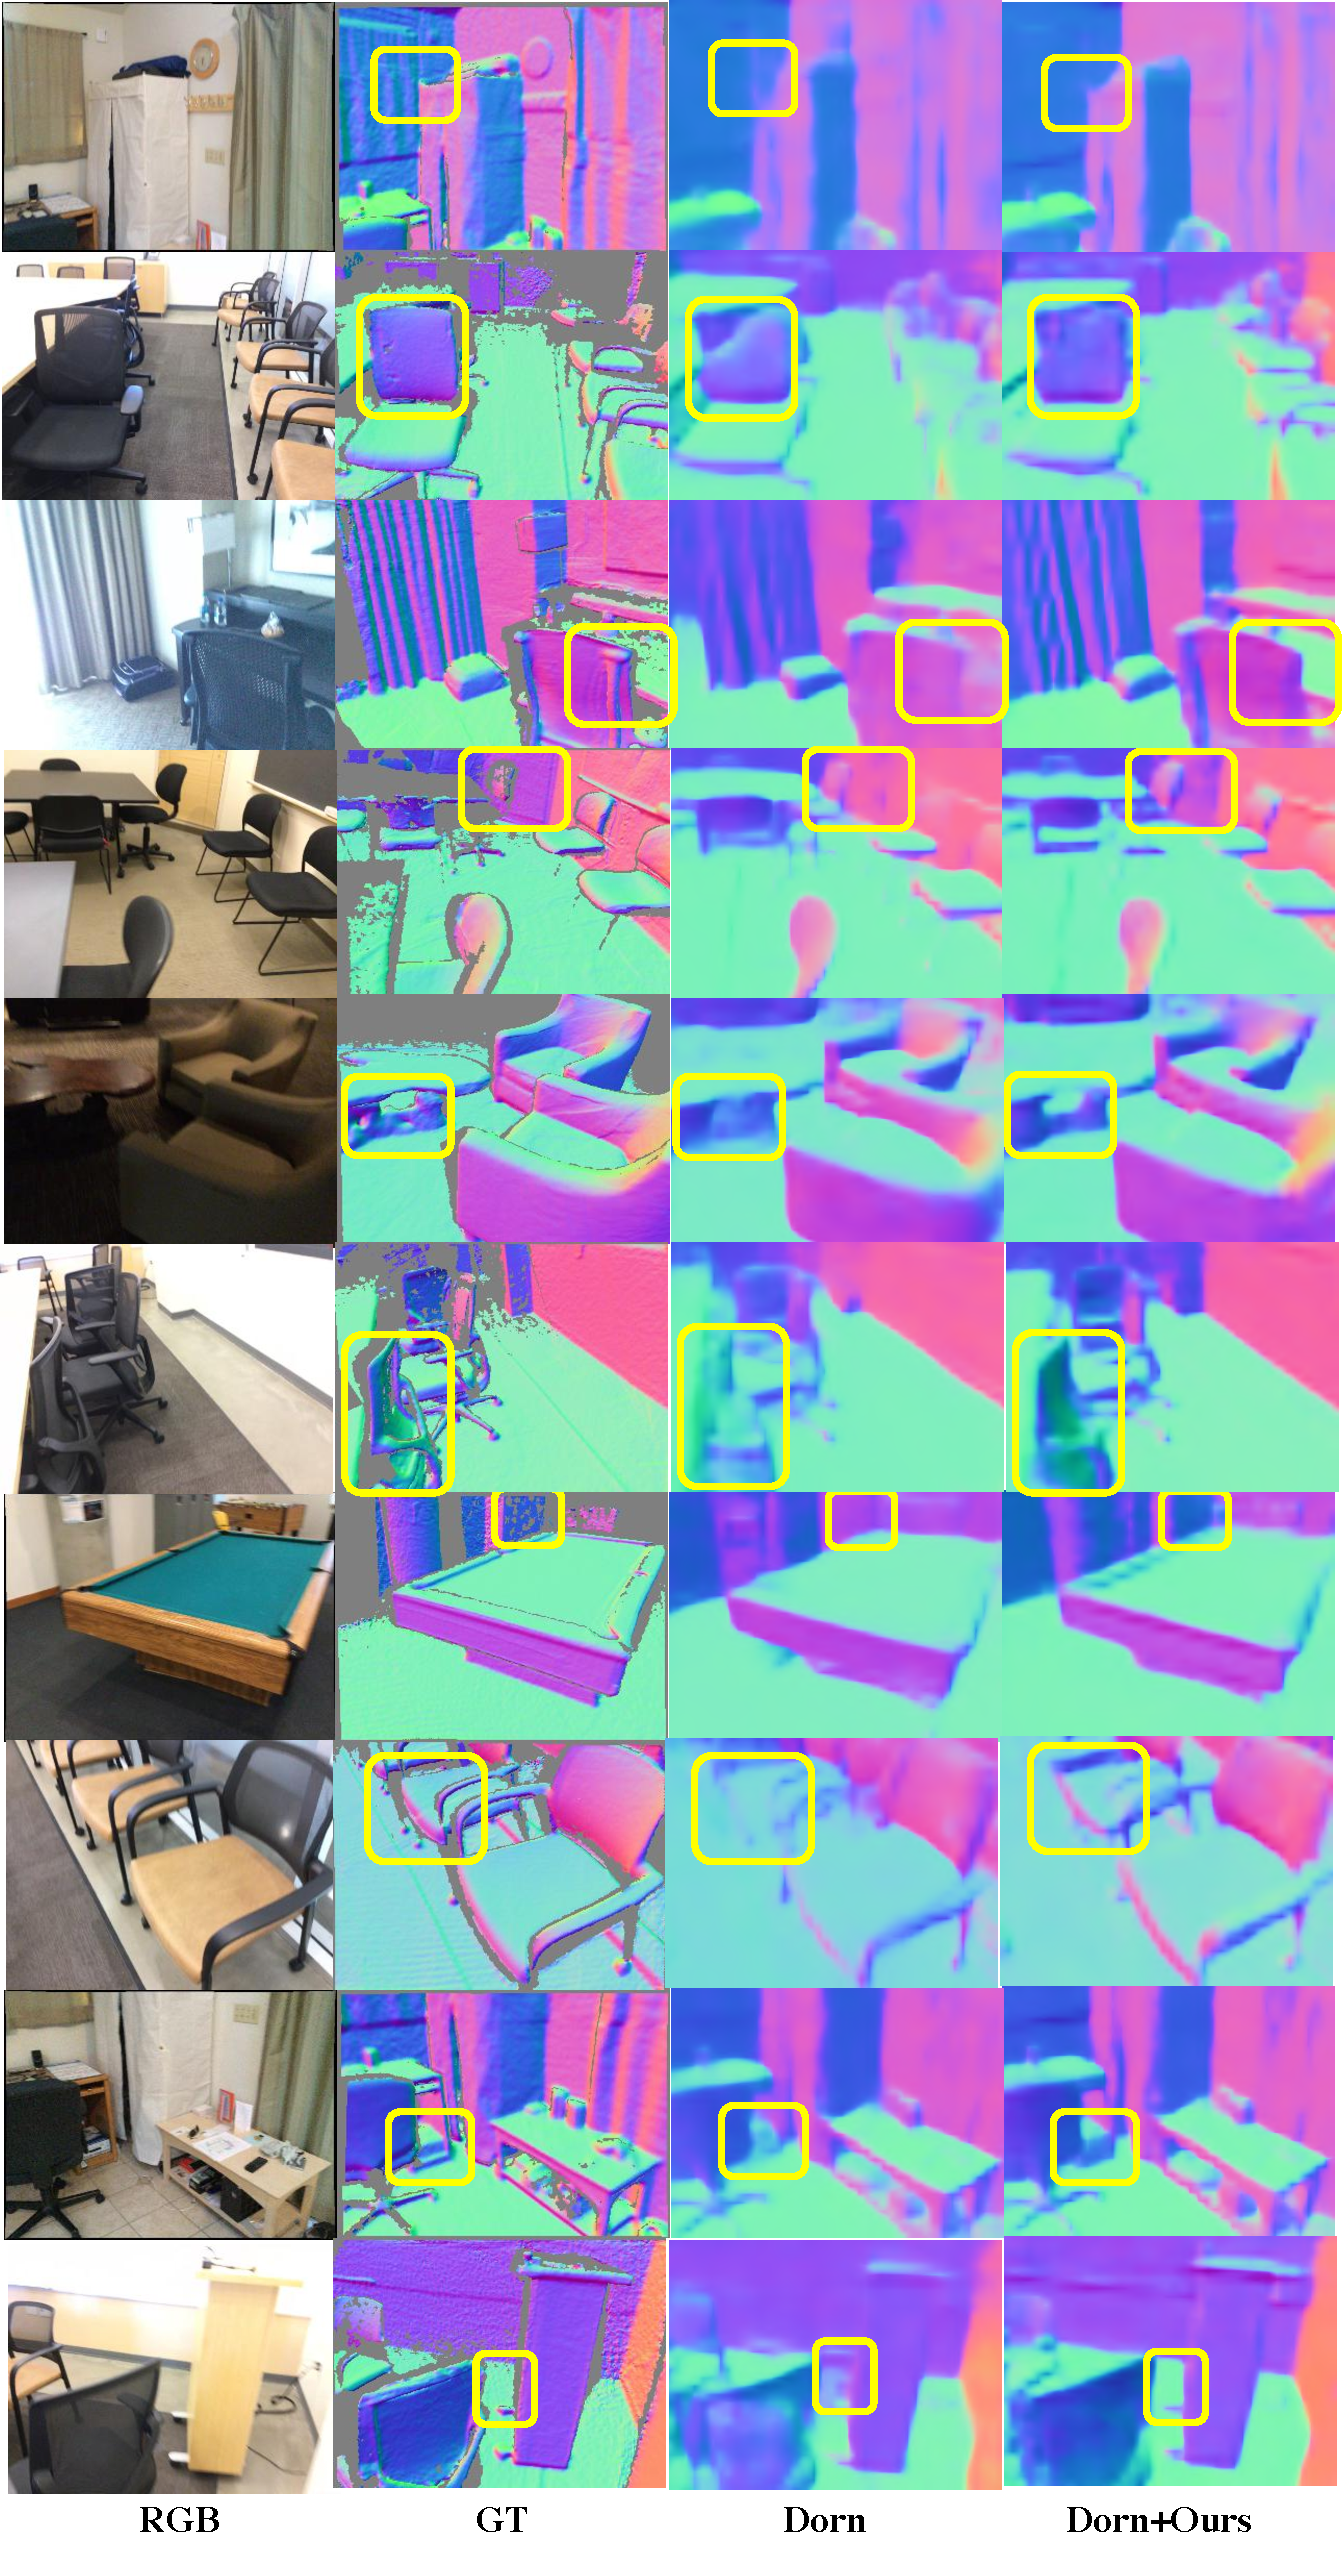
\includegraphics[width=\linewidth]{FrameNet/graph/normal-supplemental.pdf}
    \caption{Visual comparison of the results. With our joint loss, the predicted surface normals produce less errors and more details. We show more accurate prediction especially for small objects.}
    \label{fig:vis-result}
\end{minipage}
\begin{minipage}{0.49\linewidth}
    \centering
    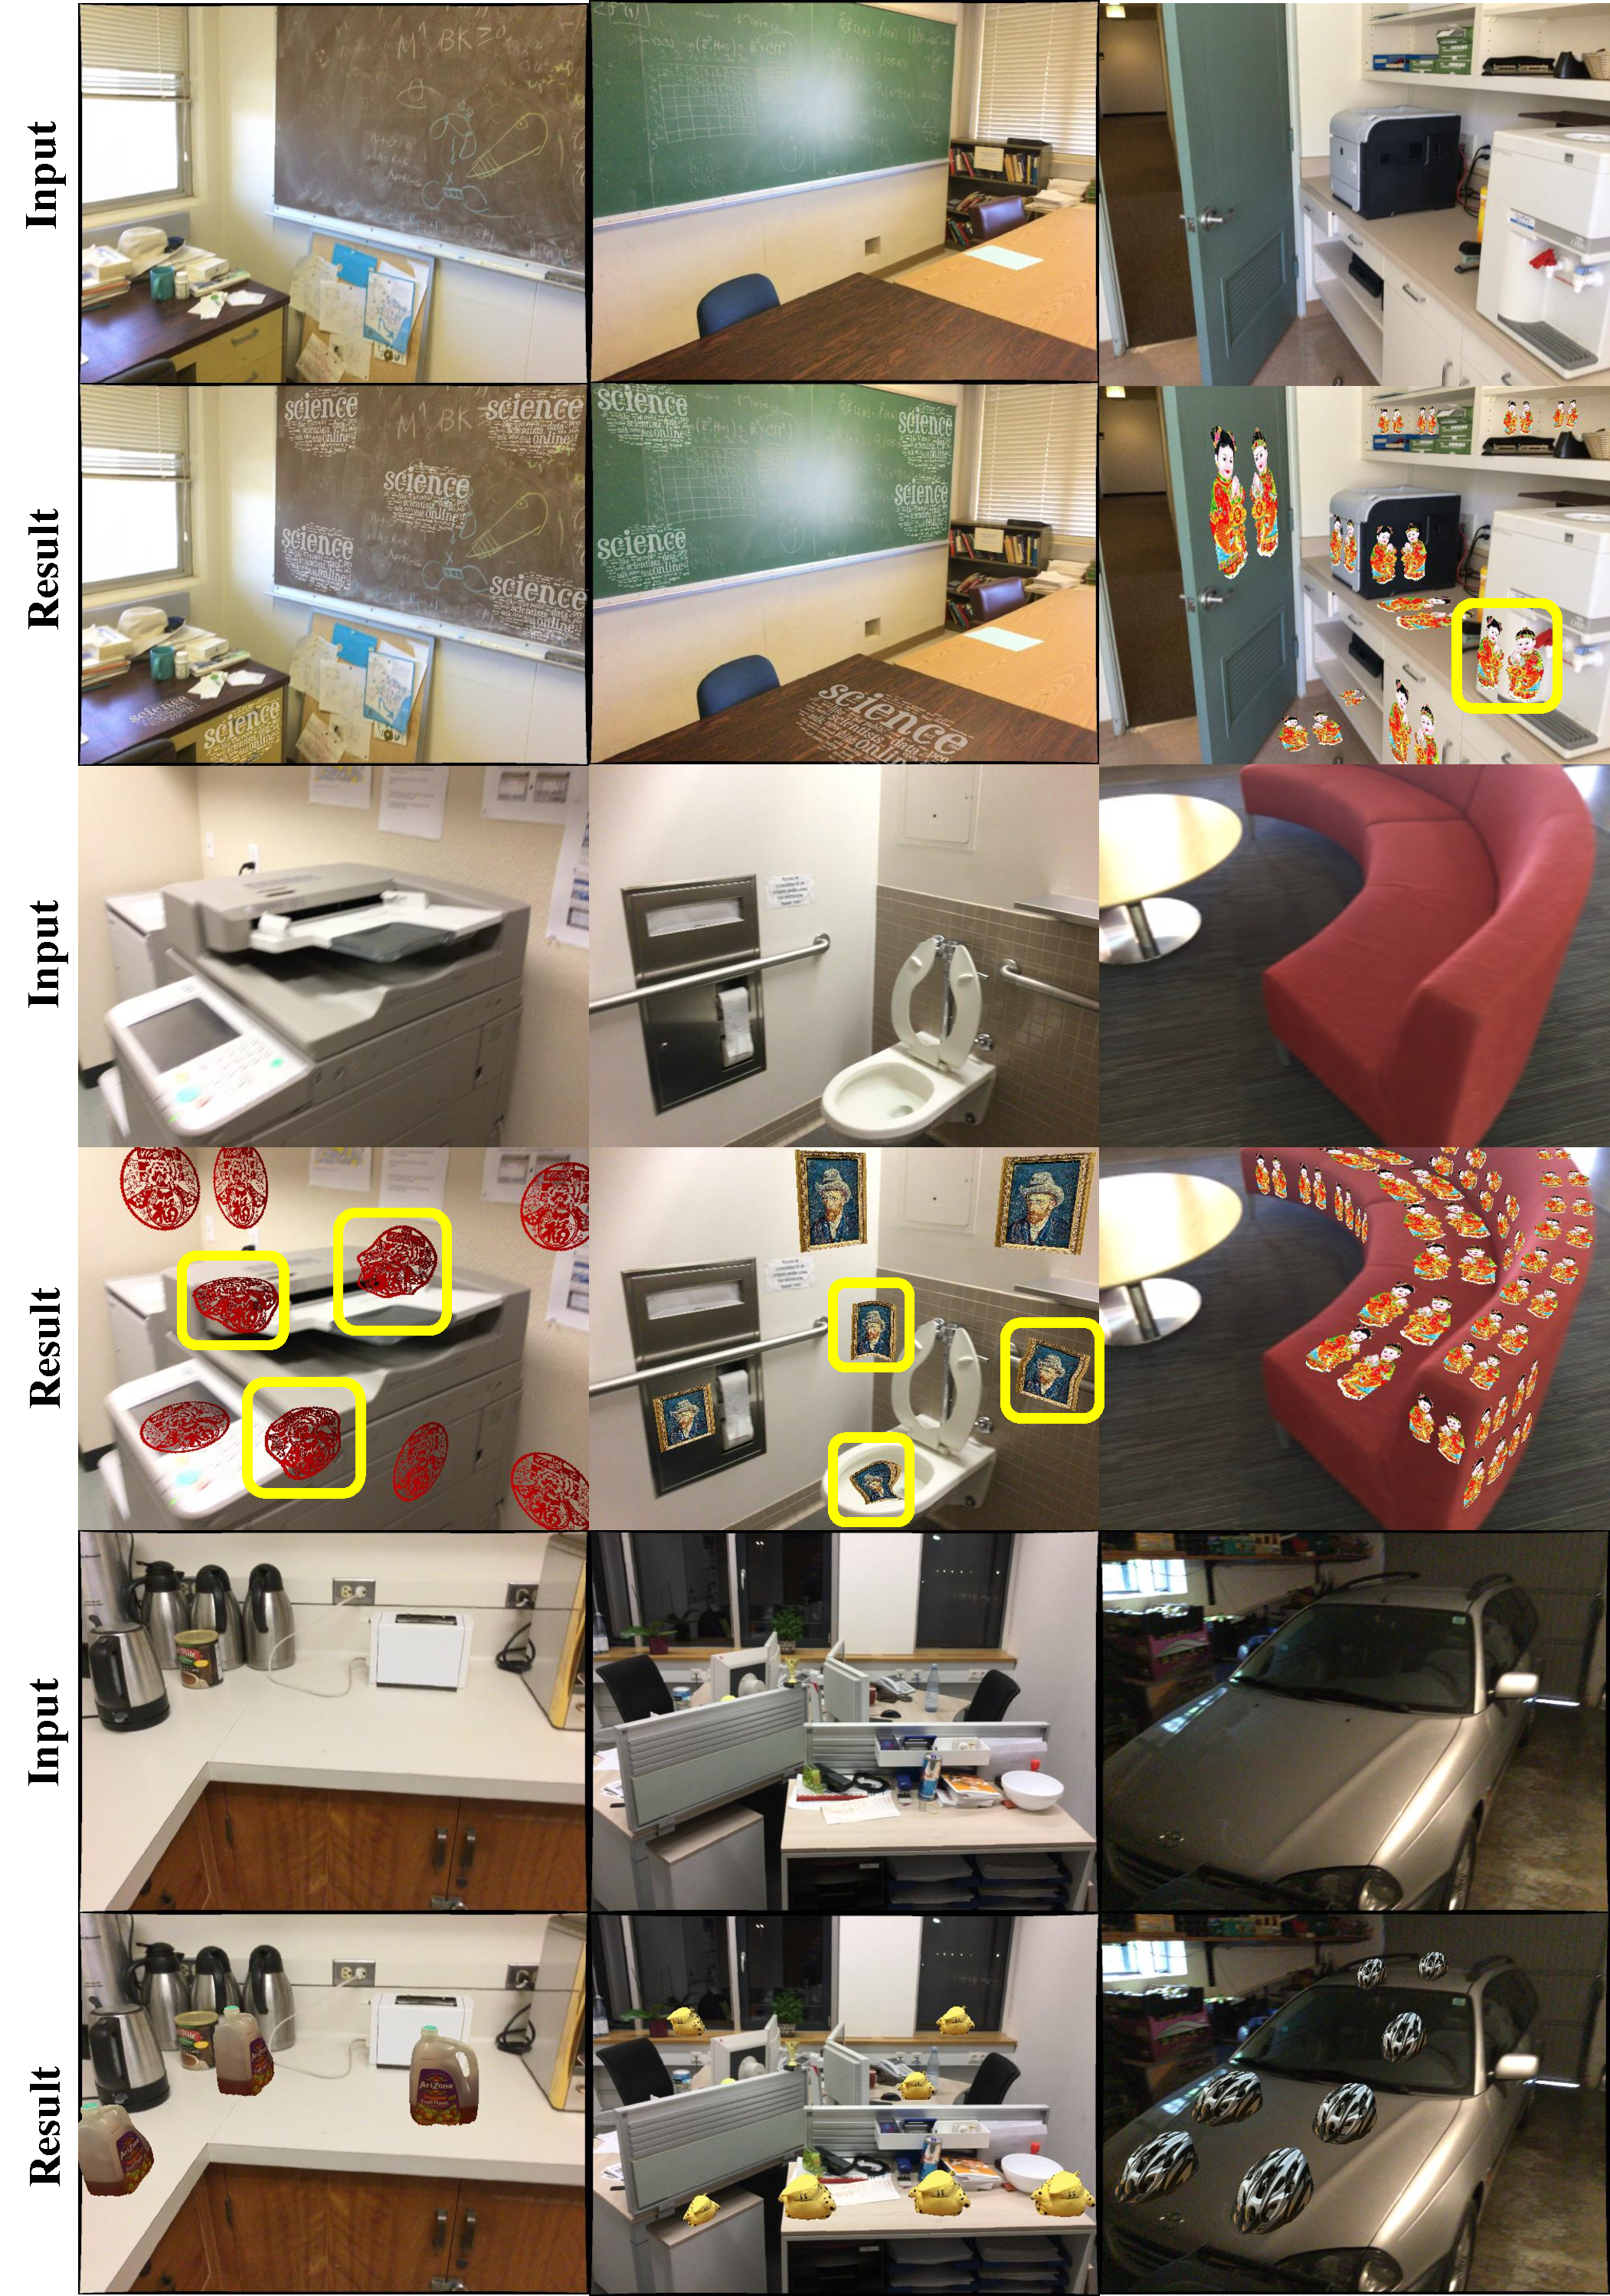
\includegraphics[width=\linewidth]{FrameNet/graph/ar-supplemental.pdf}
    \caption{Visualization of augmented reality results. We attach images in a rigid or deformable way (highlighted with yellow square), or 3D objects into the scenes. The perspectives are locally consistent with the canonical frames.}
    \label{fig:ar}
\end{minipage}
\end{figure}


\section{Visualization}
\paragraph{Surface Normal Comparison} Figure~\ref{fig:vis-result} visualizes the normal prediction using the best model w/o. our approach on both the datasets. With our approach, the errors are smaller especially at object boundaries, possibly because of the additional supervision given by the projected tangent principal directions. We show more accurate prediction, especially for small objects.

\paragraph{Visualize the tangent principal directions} We show more visualization for the projected tangent principal directions in figure~\ref{fig:vis-supplemental}. The model is trained using the Dorn~\cite{fu2018deep} with our joint loss on ScanNet~\cite{dai2017scannet}. The visualization shows a similar direction field compared to the ground truth and is consistent with human intuition.

\paragraph{Visualize the feature matching} We show more visualization for comparison between SIFT and SIFT with our perspective rectification on the DTU~\cite{aanaes2012interesting} in figure~\ref{fig:dtu-supplemental}. We produce more correct matching than SIFT does.

\paragraph{Visualize the augmented reality results} We show more examples of new elements insertion into the scene in figure~\ref{fig:ar}. The perspectives are locally consistent with the canonical frames of the geometry.
